\chapter{Methodik und experimentelles Vorgehen}
\label{Methode und Experemente}
\section{Ausgangssystem (Legacy-System \textit{Passat})}
Als Fallstudie für die experimentelle Untersuchung wurde das Legacy-System \textit{Passat} verwendet. Es handelt sich um ein internes webbasiertes
Buchungs- und Reservierungssystem, das zur Verwaltung
raumähnlicher Ressourcen in kleinen Hotels oder Pensionen
entwickelt wurde.

\textit{Passat} bietet eine Vielzahl von Funktionen, darunter die
Verwaltung von Buchungen und Reservierungen, die Speicherung
von Kundendaten sowie die Erstellung von Rechnungen. Darüber
hinaus verfügt es über ein Kalendermodul zur Darstellung
der aktuellen Raumbelegung und einen dynamischen
Preiskatalog zur Verwaltung zeitabhängiger Preise. Zusätzlich
unterstützt das System verschiedene Nutzerrollen und
Rechtestrukturen, wodurch unterschiedliche Benutzergruppen
verschiedene Funktionen des Systems nutzen können. \textit{Passat} wurde mit der Framework "Ruby on Rails"entwickelt und ist 
 und ist auf das Software Architekturmuster \textit{Model View Template (MVT)} basiert. Aufgrund seiner klar definierten Anforderungen, seiner
umfangreichen Funktionalitäten sowie der vorhandenen
Dokumentation eignet sich das System \textit{Passat} als geeignete
Fallstudie zur Untersuchung der automatischen
Systemgenerierung mithilfe von Large Language Models.

Zunächst wurden die funktionalen Anforderungen des
Legacy-Systems analysiert und strukturiert aufbereitet. Auf Basis dieser Anforderungen wurden verschiedene
Prompt-Varianten entwickelt, die anschließend in mehrere
Large Language Models (LLMs) eingegeben wurden, um neue
Implementierungen zu erzeugen.

Insgesamt wurde das System neunmal erstellt, wobei
unterschiedliche Kombinationen aus LLM-Modellen und
Prompt-Varianten verwendet wurden. Ziel war es, die
Unterschiede zwischen den generierten Systemen zu
analysieren und zu bewerten, inwieweit die ursprünglichen
Anforderungen erfüllt werden.

\section{Technische Einschränkungen beim Betrieb des \textit{Passat}-Buchungssystems}

Eine zentrale technische Herausforderung beim Betrieb des \textit{Passat} Buchungssystems ergibt sich aus dessen Charakter als Legacy-System. Die Anwendung wurde ursprünglich auf Basis des Webframeworks \textbf{"Ruby on Rails"} entwickelt und nutzt eine Vielzahl von Bibliotheken sowie externen Abhängigkeiten, die zum Zeitpunkt der Entwicklung dem Stand der Technik entsprachen. Im Laufe der Zeit wurden jedoch sowohl die Programmiersprache \textbf{"Ruby"} als auch das Framework \textbf{"Ruby on Rails"} kontinuierlich weiterentwickelt. Dies führt dazu, dass ältere Bibliotheken und Abhängigkeiten häufig nicht mehr mit aktuellen Versionen des Frameworks kompatibel sind.
Die Aktualisierung einer solchen Anwendung gestaltet sich daher oftmals schwierig. Viele der ursprünglich verwendeten Bibliotheken werden von ihren Entwicklern nicht mehr gepflegt oder stehen für neuere Framework-Versionen nicht mehr zur Verfügung. Infolgedessen müssen einzelne Abhängigkeiten manuell angepasst, ersetzt oder durch alternative Lösungen substituiert werden. Dieser Prozess ist mit einem erheblichen Entwicklungs- und Testaufwand verbunden und erhöht die Komplexität der Systemwartung.

Darüber hinaus können veraltete Software-Komponenten sicherheitsrelevante Risiken verursachen. Nicht mehr unterstützte Bibliotheken erhalten in der Regel keine Sicherheitsupdates, wodurch bekannte Schwachstellen dauerhaft bestehen bleiben. Gleichzeitig entwickeln sich auch die zugrunde liegenden Betriebssysteme kontinuierlich weiter. Insbesondere bei Linux-basierten Systemen können Änderungen an Systembibliotheken, Laufzeitumgebungen oder Sicherheitsmechanismen dazu führen, dass ältere Software-Komponenten nicht mehr lauffähig sind oder nur mit zusätzlichem Anpassungsaufwand betrieben werden können. Dadurch entsteht eine Sicherheitslücke zwischen der bestehenden Anwendung und der aktuellen Systemumgebung. Diese Problematik verdeutlicht die Herausforderungen, die beim langfristigen Betrieb von Legacy-Systemen auftreten. Die Abhängigkeit von veralteten Bibliotheken und Softwarekomponenten erschwert nicht nur die Migration auf moderne Plattformen, sondern kann zugleich die Systemsicherheit, Wartbarkeit und Zukunftsfähigkeit der Anwendung beeinträchtigen. Für das \textbf{Passat}-Buchungssystem stellt die Verwaltung und Aktualisierung solcher Abhängigkeiten daher einen wesentlichen Aspekt der technischen Weiterentwicklung dar.

\newpage
\section{Konzeptionelles Datenmodell des Buchungssystems}


\begin{figure}[ht]
    \centering
    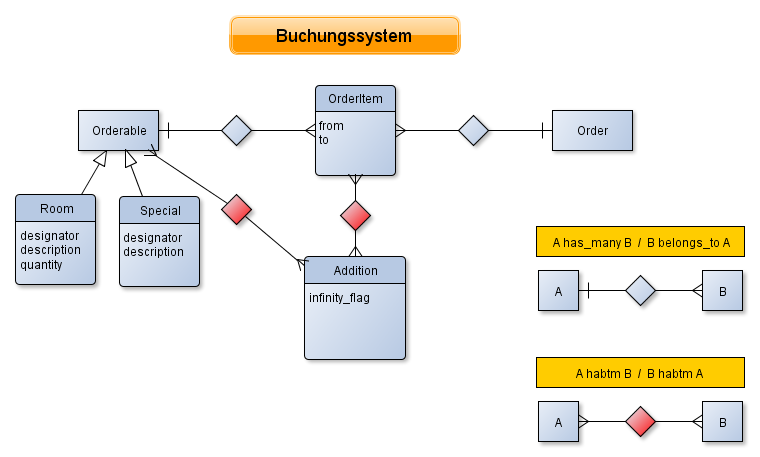
\includegraphics[width=0.8\textwidth]{images/buchungssystem.png}
  \caption{Klassendiagramm des Buchungssystems (Darstellung in Anlehnung an den Autor. \cite{Schmalz2026}).}
    \label{fig:buchungssystem}
\end{figure}

\ref{fig:buchungssystem} zeigt das Klassendiagramm des Buchungssystems. Das Modell beschreibt die zentralen Entitäten sowie deren Beziehungen und bildet die fachliche Struktur des Systems ab.

Zentrales Element ist die Entität \textit{Order}, die
einen vollständigen Buchungsvorgang repräsentiert.
Eine \textit{Order} besteht aus mehreren \textit{Order-Item},
welche jeweils einzelne Buchungseinträge mit einem
definierten Zeitraum (von/bis) darstellen. Ein
\textit{Order-Item} beschreibt somit die konkrete Nutzung
einer Ressource innerhalb eines bestimmten Zeitraums.

Die tatsächlich buchbaren Ressourcen werden durch die
abstrakte Entität \textit{Orderable} modelliert. Diese
dient als Oberklasse für unterschiedliche Ressourcentypen,
wie beispielsweise \textit{Room} oder \textit{Special}.
Durch diese Generalisierung wird eine flexible Erweiterung
des Systems ermöglicht, da neue buchbare Objekte ohne
grundlegende Änderungen integriert werden können. Ergänzend unterstützt das Modell sogenannte
\textit{Additions}, welche optionale Zusatzleistungen
repräsentieren, die einem \textit{Order-Item} zugeordnet werden
können. Beispiele hierfür sind zusätzliche Ausstattungen
oder Serviceleistungen. Die Verfügbarkeit dieser \textit{Additions}
kann entweder begrenzt oder, im Falle entsprechender
Kennzeichnung (z.\,B: durch ein \textit{infinity\_flag}),
unbegrenzt sein.

Die Beziehungen zwischen den Entitäten folgen einem
hierarchischen Aufbau: Eine \textit{Order} aggregiert mehrere
\textit{Order-Item}, während jedes \textit{Order-Item} genau einem
\textit{Orderable} zugeordnet ist. \textit{Additions} erweitern einzelne
\textit{Order-Item} und ermöglichen eine detaillierte Modellierung
komplexer Buchungsszenarien.

Das dargestellte Modell (\ref{fig:buchungssystem}) folgt grundlegenden Prinzipien
der objektorientierten Modellierung, insbesondere der
Abstraktion, Generalisierung sowie der Aggregation und
Komposition und stellt eine zentrale Grundlage für die
funktionale Struktur des Buchungssystems dar.



\newpage
\section{Analyse der Anforderungen und Spezifikation}
Die Analyse der Anforderungen basiert auf der vorhandenen
Dokumentation des Legacy-Systems \textit{Passat}, die sowohl
eine detaillierte Anforderungsbeschreibung als auch
funktionale Spezifikationen umfasst. Da \textit{Passat} nicht
öffentlich zugänglich ist, wurden zusätzliche Informationen durch den ursprünglichen Entwickler des Systems erhoben. Der Entwickler diente dabei als fachlicher Ansprechpartner,
um Unklarheiten in der bestehenden Dokumentation zu klären
und die ursprünglichen Systemanforderungen zu validieren.
Diese Kombination aus Dokumentenanalyse und Expertenwissen
ermöglichte eine konsistente und nachvollziehbare
Rekonstruktion der Anforderungen \cite{Schmalz2026}.

Im Rahmen der Analyse wurden die Anforderungen zunächst
extrahiert und anschließend in strukturierter Form
aufbereitet. Aufgrund der teilweise heterogenen und
umfangreichen Originalbeschreibung wurden die Anforderungen
konsolidiert, zusammengefasst und in mehrere Varianten
überführt. Ziel dieser Variantenbildung war es, unterschiedliche
Darstellungsformen der Spezifikation zu erzeugen, die als
Eingabe für die Large Language Models verwendet werden können. Dabei wurden die ursprünglichen funktionalen Anforderungen
nicht verändert, sondern ausschließlich in strukturierter und
für die weitere Verarbeitung geeigneter Form dargestellt.

\section{Systemarchitektur des Legacy-Systems \textit{Passat}}

Das Legacy-System \textit{Passat} basiert auf dem Architekturmuster
\textit{Model-View-Controller (MVC)}. Dieses Entwurfsmuster
unterteilt
die Anwendung in die drei Schichten \textit{Model}, \textit{View} und
\textit{Controller} und ermöglicht dadurch eine klare Trennung zwischen
Datenhaltung, Geschäftslogik, Präsentation und Anwendungssteuerung. Durch
diese Aufteilung werden die Verantwortlichkeiten einzelner Komponenten
eindeutig definiert, wodurch die Wartbarkeit, Erweiterbarkeit und
Nachvollziehbarkeit der Anwendung verbessert werden.

Die \textit{Model}-Struktur bildet die fachliche Grundlage des Systems und repräsentiert die zentralen Geschäftsobjekte sowie deren Beziehungen. Die Modelle verwalten die persistenten Daten und kapseln gleichzeitig wesentliche Teile der Geschäftslogik ab. Ihre Struktur orientiert sich an den zentralen Geschäftsprozessen der Anwendung und umfasst unter anderem Entitäten wie Kunden, Bestellungen, Belegungen, Rechnungen, Dienstleistungen, Räume sowie Benutzer. Über definierte Beziehungen zwischen den einzelnen Modellen werden komplexe fachliche Zusammenhänge konsistent abgebildet. Darüber hinaus enthalten die Modelle Validierungsmechanismen und fachliche Regeln, welche die Integrität der Anwendungsdaten sicherstellen. Durch diese klare Strukturierung\- 
konzentriert sich die Modelschicht auf die Verwaltung der fachlichen Informationen und bildet das Fundament für die übrigen Komponenten der Anwendung.

Die \textit{View}-Struktur übernimmt die Präsentation der Anwendungsdaten und stellt die Schnittstelle zwischen System und Benutzer dar. Die Ansichten sind entsprechend der funktionalen Organisation des Systems aufgebaut und bieten für die einzelnen Geschäftsobjekte geeignete Oberflächen zur Anzeige, Erstellung und Bearbeitung der Daten. Wiederverwendbare \textit{Layouts} und \textit{Partials} sorgen dabei für eine konsistente Gestaltung der Benutzeroberfläche und reduzieren redundante Implementierungen. Neben den klassischen HTML-Templates existieren spezialisierte \textit{Views} zur Erzeugung von PDF-Dokumenten sowie zur Bereitstellung strukturierter Ausgabeformate für Berichte und Auswertungen. Die konsequente Trennung der Darstellungslogik von der Geschäftslogik trägt wesentlich zur Wartbarkeit und Erweiterbarkeit der Benutzeroberfläche bei.

Die \textit{Controller}-Struktur folgt einem klar modularisierten Aufbau, bei dem einzelne funktionale Bereiche durch spezialisierte Steuereinheiten realisiert werden. Zentraler Bestandteil ist der \textit{ApplicationController}, welcher als Basisklasse für alle weiteren dient und grundlegende Funktionen wie Authentifizierung, Autorisierung, Fehlerbehandlung sowie allgemeine Mechanismen zur Filterung, Sortierung und Pagination bereitstellt. Durch diese zentrale Kapselung werden wiederkehrende Funktionalitäten vereinheitlicht und Redundanzen vermieden.

Die übrigen Steuereinheiten sind entsprechend den fachlichen Anforderungen des Systems organisiert. Im Bereich der Benutzer- und Rechteverwaltung übernehmen \textit{Controller} wie z.B.: \textit{SessionsController}, \textit{UsersController}, \textit{GroupsController} die Verwaltung von Benutzern, Gruppen und Berechtigungen und bilden damit die Grundlage des rollenbasierten Zugriffskontrollsystems. Die Kernprozesse des Systems werden durch \textit{Controller} für Kunden, Bestellungen und Bestellpositionen realisiert. Ergänzend existieren spezialisierte \textit{Controller} für individuelle Positionen und Kommentare, welche den Funktionsumfang des Buchungssystems erweitern.

Ein weiterer zentraler Funktionsbereich betrifft die Verwaltung von Belegungen. Hier übernehmen entsprechende \textit{Controller} die Verarbeitung von Belegungsdaten sowie deren Visualisierung und schaffen die Verbindung zwischen Bestellungen und der späterer Abrechnung. Das Rechnungswesen wird durch \textit{Controller} für Rechnungen und Rechnungspositionen unterstützt, die sowohl die Erstellung als auch die Verwaltung abrechnungsrelevanter Informationen ermöglichen. Ergänzend existieren spezialisierte \textit{Controller} zur Erstellung von PDF-Dokumenten. Weitere Komponenten übernehmen Aufgaben wie die Verwaltung von Dienstleistungen und Preisen, die Modellierung räumlicher Strukturen, statistische Auswertungen sowie die Verwaltung systemweiter Einstellungen und Konfigurationen.

Die Analyse der Systemarchitektur zeigt, dass das Legacy-System \textit{Passat} das MVC-Architekturmuster konsequent umsetzt. Die fachliche Logik ist in den Modellen gekapselt, die Präsentation erfolgt innerhalb der \textit{Views} und die \textit{Controller} koordinieren den Ablauf der Geschäftsprozesse sowie die Kommunikation zwischen den einzelnen Schichten. Gleichzeitig folgt jede Ebene einer funktionalen Modularisierung, wodurch eine hohe Kohäsion innerhalb der Komponenten und eine geringe Kopplung zwischen den einzelnen Systembereichen erreicht werden. Diese Architektur erleichtert die Wartung des Legacy-Systems, unterstützt die Analyse der bestehenden Softwarestruktur und schafft eine geeignete Grundlage für zukünftige Erweiterungen und Modernisierungsmaßnahmen.

\section{Prompt Engineering und Prompt-Varianten}

Die Erstellung der Softwaresysteme basiert auf dem
Einsatz von Prompt Engineering, welches die gezielte
Gestaltung von Eingaben für LLMs
beschreibt \cite{boonstra2024prompt}.

Die Prompts wurden auf Grundlage der analysierten
Systemanforderungen entwickelt. Dabei kamen insbesondere
Semantik-Prompting sowie strukturierte
Promptformulierungen zum Einsatz. Ziel war es, dem Modell
ein möglichst vollständiges Verständnis der Systemdomäne
zu vermitteln.
Die Schaffung von Programmcodes stellt eine zentrale
Anwendung von LLMs dar. Effektive Prompts bestehen dabei
aus einer klaren Aufgabenbeschreibung, einer strukturierten
Darstellung der Logik sowie einer expliziten Aufforderung
zur Erzeugung des Codes.

Eine aktuelle Studie untersucht den Einfluss der Eingaberepräsentation auf
die Reasoning-Fähigkeiten großer Sprachmodelle (LLMs).
Die Autoren schlagen mit  \textit{Code-Prompting} einen Ansatz vor, 
bei dem Aufgaben in natürlicher Sprache zunächst in eine Code-Darstellung überführt werden.
Anschließend wird das Modell direkt mit dieser strukturierten
Repräsentation konfrontiert, ohne den erzeugten Code auszuführen.
Die Ergebnisse zeigen, dass diese Methode die Leistung verschiedener
LLMs bei logischen und konditionalen \textit{Reasoning}-Aufgaben deutlich verbessert.
Die Autoren führen dies darauf zurück, dass die Code-Darstellung insbesondere
das Nachverfolgen von Zuständen und Entitäten sowie logischer Schlussfolgerungen erleichtert \cite{puerto-etal-2024-code}.


Darüber hinaus ist die Validierung des generierten Codes
von entscheidender Bedeutung. Hierzu wurde der erzeugte
Code gespeichert, ausgeführt und hinsichtlich seiner
Funktionalität überprüft.

\section{Definition der Prompt-Varianten und eingesetzte LLM-Modelle}

Zur Untersuchung wurden drei Prompt-Varianten mit
unterschiedlichem Komplexitätsgrad definiert (siehe Anhang):

\begin{itemize}
\item \textbf{Prompt 1}: Einfacher Basis-Prompt ohne Struktur
\item \textbf{Prompt 2}: Strukturierter Prompt mit Kontextinformationen
\item \textbf{Prompt 3}: Erweiterter Prompt mit Role Prompting
\end{itemize}

Ziel ist es, den Einfluss der Promptstruktur auf die
Qualität der generierten Systeme zu analysieren. Die vollständigen und tatsächlich verwendeten Prompts zur
Generierung der Softwaresysteme sind aus Gründen der
Nachvollziehbarkeit im Anhang dokumentiert.


In dieser Arbeit wurden folgende Modelle verwendet:

\begin{itemize}
\item \textbf{GPT 5.2}
\item \textbf{Gemini 3.1 Pro}
\item \textbf{GPT-5.3-Codex}

\end{itemize}

Diese Modelle wurden ausgewählt, um unterschiedliche Fähigkeiten moderner LLMs abzudecken. Alle eingesetzten Modelle basieren auf der Transformer-Architektur, unterscheiden sich jedoch hinsichtlich ihrer Spezialisierung und ihres Anwendungsschwerpunkts.

\textbf{GPT 5.2} stellt ein generalistisches Sprachmodell dar, das für eine breite Palette von Aufgaben der natürlichen Sprachverarbeitung eingesetzt wird. Dazu zählen u.a. Texterstellung, Zusammenfassung, semantische Analyse sowie logisches Schlussfolgern. Das Modell zeichnet sich durch eine hohe Kontextverarbeitungskapazität und robuste Generalisierungsfähigkeit aus.

\textbf{Gemini 3.1 Pro} ist ein multimodales Modell, das neben einfachem Text auch weitere Datentypen wie Bilder und strukturierte Informationen verarbeiten kann. Der Fokus liegt auf der Integration und Analyse unterschiedlicher Informationsquellen. Dadurch eignet sich das Modell besonders für komplexe Aufgabenstellungen, bei denen ein kontextübergreifendes Verständnis erforderlich ist.

\textbf{GPT-5.3-Codex} ist ein auf Softwareentwicklung spezialisiertes Modell. Es wurde gezielt auf große Mengen von Quellcodes sowie technische Dokumentationen trainiert und ist insbesondere für Aufgaben wie Codeerzeugung, Codeanalyse und automatische Vervollständigung geeignet. Durch seine detaillierte Mustererkennung formaler Sprache ermöglicht es eine effiziente Unterstützung im Entwicklungsprozess sowie die Übersetzung von natürlichsprachlichen Anforderungen im ausführbaren Code.

Durch die Kombination dieser drei Modelle wird sowohl eine breite Abdeckung allgemeiner Sprachverarbeitungsaufgaben als auch eine Spezialisierung auf technische und multimodale Anwendungsfälle erreicht. Dies ermöglicht eine differenzierte Analyse und Nutzung der jeweiligen Modellstärken im Rahmen dieser Arbeit.



\section{Technische Umgebung}


Die Durchführung der Experimente erfolgte in mehreren
Schritten. Zunächst wurden die definierten Prompts in die
jeweiligen LLM-Systeme eingegeben, um ein vollständiges
Softwaresystem zu generieren. Der generierte Code wurde anschließend lokal gespeichert
und in einer geeigneten Entwicklungsumgebung ausgeführt.
Dabei wurden insbesondere Python und das Webframework
Django verwendet. Im nächsten Schritt erfolgte die funktionale Überprüfung
der generierten Systeme. Hierbei wurden zentrale
Anwendungsfälle getestet, wie die Erstellung von Kunden,
die Verwaltung von Buchungen sowie die Interaktion über
die Benutzeroberfläche. Abschließend wurden die Ergebnisse dokumentiert und auf
Basis der definierten Evaluationskriterien bewertet, um
eine vergleichende Analyse der verschiedenen Modelle und
Prompt-Varianten zu ermöglichen.




Zur Entwicklung und Auswertung wurde eine integrierte
Entwicklungsumgebung verwendet, die eine direkte
Interaktion mit den LLMs sowie die Ausführung des Codes
ermöglichte. Im vorliegenden Fall wurde die integrierte Entwicklungsumgebung \textbf{Visual Studio Code (VS Code)}  als Integrated Development Environment (IDE) verwendet.

Als isolierte Laufzeitumgebung für das Projekt wurde das Python-Tool \textbf{venv-Umgebung (Virtual Enviroment)} angenommen. 


\chapter{Evaluationskriterien}
\label{chapter-evaluation-criteria}

Zur Bewertung der generierten Systeme wurden vier zentrale Kategorien von Evaluationskriterien definiert:
\begin{itemize}
    \item Funktionale Kriterien
    \item Technische Kriterien
    \item Integrationskriterien
    \item Leistungskriterien
\end{itemize}

Ziel dieser Bewertung ist eine strukturierte und nachvollziehbare Analyse der Qualität, Zuverlässigkeit und Leistungsfähigkeit der entwickelten Systeme.

Die \textbf{funktionalen Kriterien} überprüfen insbesondere die korrekte Umsetzung der definierten Anforderungen und Geschäftsprozesse. Dabei wird bewertet, ob die implementierten Funktionen erwartungsgemäß arbeiten und die vorgesehenen Anwendungsfälle vollständig unterstützen.

Die \textbf{technischen Kriterien} fokussieren auf interne Qualitätsmerkmale des Systems. Hierzu zählen unter anderem die Codequalität, die Architektur, die Wartbarkeit, die Datenmodellierung sowie die Einhaltung technischer Standards und bewährter Vorgehensweisen (Best Practices).

Die \textbf{Integrationskriterien} bewerten das Zusammenspiel einzelner Systemkomponenten innerhalb realistischer Benutzerabläufe. Dabei wird geprüft, ob Frontend, Backend, Datenbank und Benutzeroberfläche konsistent zusammenarbeiten und typische Workflows fehlerfrei ausgeführt werden können.

Die \textbf{Leistungskriterien} analysieren die Effizienz und Stabilität des Systems. Bewertet werden insbesondere Antwortzeiten, Speicherverbrauch, Skalierbarkeit sowie das Verhalten des Systems unter wiederholten oder komplexen Anfragen.

Die Bewertung der Leistungskriterien mittels Performancetests ist insbesondere bei Systemen mit einer hohen Anzahl gleichzeitiger Benutzer von großer Bedeutung. Solche Tests ermöglichen die Analyse der Ressourcenauslastung sowie die Identifikation potenzieller Leistungsengpässe unter Lastbedingungen. Im Rahmen dieser Arbeit wurde auf die Durchführung von Performancetests verzichtet, da das untersuchte System derzeit nur von einer begrenzten Anzahl von Benutzern verwendet wird. Darüber hinaus wäre für eine aussagekräftige Bewertung der Systemleistung der Einsatz spezialisierter Performance-Testwerkzeuge erforderlich gewesen. Aus diesem Grund wurden die Leistungskriterien nicht in die Evaluation einbezogen.

Die Bewertung erfolgt anhand strukturierter Test-Checklisten und eines Punktesystems, um eine objektive und vergleichbare Analyse der generierten Systeme zu ermöglichen.

\section{Effizienzsteigerung durch strukturierte Prompts bei Large Language Models, LLMs}
Große Sprachmodelle (\textit{Large Language Models}, LLMs) werden zunehmend für komplexe und wissensintensive Aufgabenbereiche, insbesondere im Kontext der Softwareentwicklung, der automatisierten Anforderungsanalyse sowie weiterer informationsverarbeitender Prozesse eingesetzt, wobei die Qualität der durch das Modell erzeugten Ergebnisse in erheblichem Maße von der Struktur, Präzision und semantischen Gestaltung der Eingabeaufforderung (\textit{Prompt}) abhängig ist.

Insbesondere bei umfangreichen und inhaltlich stark verdichteten Eingaben zeigt sich, dass eine systematische Zerlegung der Gesamtaufgabe in mehrere kleinere, klar definierte und logisch voneinander abgegrenzte Teilaufgaben deutlich effizienter und zuverlässiger ist als die Verwendung eines einzelnen, komplex formulierten Prompts, da hierdurch die Verarbeitungsschritte transparenter und besser kontrollierbar gestaltet werden können \cite{cot10_1145_3690635} .

Ein zentrales Problem bei langen und informationsreichen Eingaben besteht in der ungleichen Gewichtung einzelner Informationen innerhalb des Sprachmodells, wodurch relevante Inhalte teilweise in den Hintergrund treten können, während weniger bedeutsame Informationen überproportional berücksichtigt werden, was in vielen Fällen zu unvollständigen, inkonsistenten oder fehlerhaften Ergebnissen führt \cite{liu2023lost}.
Darüber hinaus führt eine hohe Informationsdichte innerhalb eines Prompts zu einer erhöhten kognitiven Komplexität der zu verarbeitenden Aufgabe insbesondere, wenn mehrere unterschiedliche Anforderungen oder Verarbeitungsschritte simultan berücksichtigt werden müssen, da in solchen Situationen sogenannte Interferenzeffekte auftreten können, bei denen verschiedene Teilaufgaben miteinander konkurrieren und somit die begrenzten Verarbeitungsressourcen des Modells beanspruchen \cite{cot10_1145_3690635}.

Die Aufteilung komplexer Prozesse in mehrere aufeinanderfolgende Verarbeitungsschritte, beispielsweise in Form einer Analyse-, Validierungs- und anschließenden Implementierungsphase (\textit{Analyse} $\rightarrow$ \textit{Validierung} $\rightarrow$ \textit{Implementierung}), ermöglicht hingegen eine deutlich klarere Fokussierung auf die jeweilige Teilaufgabe und verbessert dadurch sowohl die Nachvollziehbarkeit als auch die Konsistenz der generierten Ergebnisse.

Die beschriebene Vorgehensweise ähnelt dem in der Literatur häufig diskutierten Prinzip der Aufgabenzerlegung (*Task Decomposition*), bei dem komplexe Probleme in mehrere kleinere und besser handhabbare Teilaufgaben unterteilt werden. Im Gegensatz zum klassischen \textit{Chain-of-Thought (CoT)} Prompting, bei dem das Sprachmodell innerhalb einer einzelnen Anfrage Zwischenschritte zur Lösung einer Aufgabe generiert, erfolgt in dieser Arbeit die Zerlegung auf Ebene des Softwareentwicklungsprozesses. Die einzelnen Entwicklungsphasen werden nacheinander durchgeführt und nach jedem Schritt überprüft, bevor mit der nächsten Phase fortgefahren wird. Dadurch kann die Komplexität der Gesamtaufgabe reduziert und die Konsistenz der generierten Software verbessert werden.

Aktuelle Forschungsarbeiten zeigen jedoch, dass herkömmliche CoT-Ansätze trotz ihrer verbesserten Problemlösungsfähigkeiten weiterhin Einschränkungen hinsichtlich Genauigkeit und Konsistenz aufweisen können, insbesondere bei komplexen Aufgaben der Codegenerierung \cite{cot10_1145_3690635}.

Vor diesem Hintergrund wurde mit den sogenannten \textit{Structured Chain-of-Thoughts (SCoTs) } ein Ansatz vorgestellt, der strukturierte Denkprozesse explizit an den Prinzipien des strukturierten Programmierens orientiert, indem sequenzielle, verzweigende sowie iterative Programmstrukturen bereits innerhalb der \textit{reasoning steps} berücksichtigt werden.
Durch die explizite Einbindung solcher strukturellen Muster wird das Sprachmodell dazu angeleitet, logisch konsistenter und besser organisierte Zwischenschritte zu erzeugen, wodurch die Qualität und Robustheit der generierten Ergebnisse signifikant verbessert werden kann.
Ein weiterer wesentlicher Vorteil dieser Methodik besteht darin, dass Zwischenergebnisse sichtbar gemacht und separat überprüft werden können, wodurch potenzielle Fehler oder Inkonsistenzen bereits in frühen Phasen des Verarbeitungsprozesses identifiziert und korrigiert werden können.
Insgesamt trägt die strukturierte Zerlegung komplexer Aufgabenstellungen somit wesentlich zur Verbesserung der Leistungsfähigkeit, Nachvollziehbarkeit und Zuverlässigkeit großer Sprachmodelle bei.

\section{Ableitung der Evaluationskriterien aus bestehenden Testfällen}

Die Evaluationskriterien dieser Arbeit wurden nicht ausschließlich
theoretisch definiert, sondern zusätzlich aus den vorhandenen
Testfällen des Legacy-Systems abgeleitet. Die bestehenden Tests
stellen dabei eine implizite Beschreibung der funktionalen und
technischen Anforderungen des ursprünglichen Buchungssystems dar.

Jeder Testfall überprüft ein bestimmtes erwartetes Verhalten des
Systems und beschreibt somit indirekt, welche Eigenschaften das
System erfüllen muss. Durch die Analyse der Testfälle konnten
konkrete Evaluationskriterien identifiziert und systematisch
strukturiert werden.

Das grundlegende Vorgehen basiert auf der Überführung von
Testfällen in fachliche und technische Qualitätsanforderungen.
Dabei wird aus jedem Test die folgende Beziehung abgeleitet:

\begin{center}
Testfall $\rightarrow$ erwartetes Verhalten $\rightarrow$
Evaluationskriterium
\end{center}

Beispielsweise kann aus einem Test, der prüft, ob ungültige
Filteroperatoren erkannt und mit einer Fehlermeldung abgelehnt
werden, das folgende Evaluationskriterium abgeleitet werden:

\begin{quote}
Das System muss ungültige Filteroperatoren erkennen und mit
einem Syntaxfehler ablehnen.
\end{quote}

Auf diese Weise wurden die bestehenden Tests analysiert und
in mehrere Kategorien von Evaluationskriterien überführt.

Die abgeleiteten Evaluationskriterien ermöglichen eine strukturierte
und nachvollziehbare Bewertung der generierten Systeme.
Zur quantitativen Analyse wurde zusätzlich ein
Bewertungsschema verwendet, bei dem jedes Kriterium
auf einer Skala bewertet wird:

\begin{itemize}
    \item 0 = nicht erfüllt
    \item 1 = teilweise erfüllt
    \item 2 = vollständig erfüllt
\end{itemize}

Durch dieses Vorgehen entsteht ein systematischer
Evaluationskatalog, der sowohl funktionale als auch
technische Aspekte der generierten Softwaresysteme
berücksichtigt und eine vergleichbare Bewertung der
verschiedenen LLMs ermöglicht.

\section{Bedeutung der Test-Checklisten für die Systembewertung}

Softwaretests dienen der systematischen Überprüfung von Funktionalität, Qualität und Zuverlässigkeit eines Softwaresystems. Durch strukturierte Testverfahren können Fehler frühzeitig erkannt und die Einhaltung definierter Anforderungen validiert werden \cite{Ammann2017}. 
Insbesondere Checklisten und standardisierte Testfälle verbessern die Nachvollziehbarkeit, Wiederholbarkeit und Wartbarkeit von Softwaretests \cite{ISTQB2018}.

Die im Rahmen dieser Arbeit verwendeten Test-Checklisten dienen der systematischen Bewertung der funktionalen, technischen und integrativen Anforderungen des entwickelten Systems. Durch die strukturierte Auflistung einzelner Prüfkriterien wird sichergestellt, dass alle relevanten Komponenten und Geschäftsprozesse vollständig und reproduzierbar getestet werden.
\newpage
Die Bewertung orientiert sich an den folgenden Kriterienbereichen. Die Checklisten erfüllen dabei mehrere zentrale Aufgaben:

\begin{itemize}

    \item[] \textbf{Funktionale Kriterien}

    \item \textbf{Allgemeine Funktionalität}: Prüft, ob die Anwendung eine nutzbare
    Oberfläche mit Formularen, Navigation und konsistenter URL-Struktur 
    bereitstellt. Darüber hinaus werden erweiterte Funktionen wie Sortierung, 
    Filterung, Pagination sowie vollständige CRUD-Operationen und eine 
    geeignete Fehlerbehandlung bewertet. Ergänzend wird geprüft, ob 
    Login/Logout, Session-Handling, Fehlermeldungen bei ungültigem Login 
    sowie der Schutz geschützter Bereiche korrekt umgesetzt sind.

    \item \textbf{Geschäftsobjekte und CRUD-Funktionalität}: Prüft, ob zentrale 
    Geschäftsobjekte wie \textit{Customers, Orders, Rooms, Tasks und Invoices} 
    vollständig umgesetzt wurden. Dabei wird bewertet, ob Listendarstellungen, 
    Detailansichten, Erstellen, Aktualisieren und Löschen je Ressource korrekt 
    implementiert sind. Zusätzlich werden verschachtelte Routen, 
    Kundenbindungsregeln, Stornofunktionen sowie 404-Fehlerbehandlung geprüft.

    \item \textbf{Erweiterte Domänenfunktionen}: Prüft, ob erweiterte Domänenobjekte 
    wie \textit{\textit{Order Items, Occupancy Items, Services, Kommentare und Room Locations}} 
    vollständig als CRUD-Ressource implementiert wurden. Bewertet werden 
    zudem Statusbehandlung, Belegungseinträge, Rechnungspositionen, 
    Generierung aus Bestellungen sowie optional polymorphe Ziele bei 
    Kommentaren und freie Räume in einem definierten Zeitraum.

    \item \textbf{Benutzer- und Rechteverwaltung}: Prüft, ob Benutzer- und 
    Rollenmodelle vorhanden sind und ob eine vollständige Rechteverwaltung 
    und Autorisierung umgesetzt wurden. Hierzu zählen die Gruppenverwaltung, 
    die Berechtigungszuweisung sowie die nachweisbare Wirkung dieser 
    Berechtigungen im System.

    \item[] \textbf{Technische Kriterien}

    \item \textbf{Modell-Validierungen und Geschäftslogik}: Prüft, ob Modellvalidierungen und 
    Geschäftsregeln sowie technische Qualitätssicherungsmechanismen 
    vollständig umgesetzt wurden. Bewertet werden insbesondere 
    Modellbeziehungen, Callbacks, Löschregeln, Fachlogik sowie die korrekte 
    Fehlerzuweisung auf Unit-Test-Ebene.

    \item \textbf{Unit-Tests}: Prüft, ob automatisierte Unit-Tests generiert und 
    implementiert wurden. Dabei wird bewertet, ob die Tests HTTP-Status, 
    Datenbankkonsistenz, Fehlerfälle, verschachtelte Ressourcen, 
    Modellregeln sowie realistische Fixtures abdecken.

    \item \textbf{Codequalität und Wartbarkeit}: Prüft, ob die technische Struktur 
    nachweisbare Mechanismen zur Qualitätssicherung und Testbarkeit enthält, 
    darunter eine klare Trennung von Verantwortlichkeiten sowie eine 
    konsistente und wartbare Codebasis.

    \item[] \textbf{Integrationskriterien}

    \item \textbf{Frontend-Backend-Integration}: Prüft, ob grundlegende Interaktionen 
    zwischen Benutzeroberfläche und Backend korrekt umgesetzt sind. Bewertet 
    werden reale Nutzerabläufe über die GUI inklusive Navigation, Formularen, 
    Fehlermeldungen, Modals und Stabilität sowie ob komplexe Workflows 
    vollständig implementiert wurden.

    \item \textbf{End-to-End-Workflows}: Prüft, ob vollständige Benutzerabläufe sowie 
    automatisierte Integrationstests vorhanden sind.

\end{itemize}
Die funktionalen Kriterien bewerten die Umsetzung der fachlichen Anforderungen, der Geschäftsobjekte sowie der Benutzer- und Rechteverwaltung. Die technischen Kriterien überprüfen die Qualität der Implementierung hinsichtlich Validierungen, Geschäftslogik, automatisierter Unit-Tests und Wartbarkeit des Quellcodes. Die Integrationskriterien untersuchen das Zusammenspiel von Frontend, Backend und Datenbank sowie die korrekte Umsetzung vollständiger Benutzerabläufe.

Die Kombination aus funktionalen, technischen und Integrationskriterien ermöglicht eine umfassende und mehrdimensionale Bewertung der generierten Systeme. Während die funktionalen Kriterien die fachliche Korrektheit überprüfen, analysieren die technischen Kriterien die interne Qualität der Implementierung. Die Integrationskriterien validieren das Zusammenspiel aller Systemkomponenten innerhalb realistischer Benutzerabläufe.

Durch die Kombination dieser unterschiedlichen Kriterien entsteht eine umfassende Bewertung des Gesamtsystems hinsichtlich Funktionalität, Zuverlässigkeit, Benutzerfreundlichkeit und Leistungsfähigkeit.


Mit dieser strukturierten Vorgehensweise entsteht eine nachvollziehbare und vergleichbare Grundlage zur Bewertung der entwickelten Systeme hinsichtlich Funktionalität, Qualität, Benutzerfreundlichkeit und Leistungsfähigkeit.




\chapter{Evaluationsergebnisse}
\label{Evaluationsergebnisse}

Für jedes Experiment werden die Ergebnisse zunächst in einer zusammenfassenden Tabelle dargestellt, die einen Überblick über den Erfüllungsgrad der allgemeinen Anforderungen bietet. Darüber hinaus werden die Bewertungen der einzelnen Funktionen und Anforderungen in detaillierten Tabellen im Anhang dokumentiert. Diese Vorgehensweise ermöglicht sowohl eine kompakte Darstellung der zentralen Ergebnisse im Hauptteil der Arbeit als auch eine transparente und nachvollziehbare Analyse der einzelnen Bewertungskriterien.

Hierzu wurden drei Experimente an jedem der drei Modelle durchgeführt, die sich hinsichtlich des verwendeten Prompt-Designs unterscheiden. Im ersten Experiment wurde ein einfacher Basis-Prompt eingesetzt, um die Leistungsfähigkeit des Modells ohne weiterführende Prompt-Engineering-Techniken zu untersuchen. Das zweite Experiment verwendete einen strukturierten Prompt mit zusätzlichen Kontextinformationen und detaillierten Anforderungen. Im dritten Experiment wurde der strukturierte Prompt um eine explizite Rollendefinition erweitert, bei der das Modell die Rolle eines erfahrenen Softwarearchitekten und Full-Stack-Entwicklers einnahm.

Die Bewertung der generierten Anwendungen erfolgt anhand einer einheitlichen Checkliste, die auf den zuvor definierten funktionalen, technischen, integrationsbezogenen Kriterien basiert. 

Durch die schrittweise Erhöhung der Prompt-Komplexität soll untersucht werden, inwieweit eine präzisere Aufgabenbeschreibung die Qualität, Vollständigkeit und Konsistenz der generierten Softwarelösung beeinflusst. Besonderes Interesse gilt dabei der Umsetzung funktionaler Anforderungen, der Einhaltung technischer Qualitätskriterien sowie der Berücksichtigung von Integrations- und Performance-Aspekten.

Anschließend werden die Resultate miteinander verglichen und hinsichtlich des Einflusses der unterschiedlichen Prompt-Strategien auf die Qualität der generierten Softwarelösungen diskutiert.

Alle Experimente befinden sich zusammen mit dem gesamten generierten Projekt und den zugehörigen Prompts im \textit{GitLab-Repository} der Universitätswebseite (siehe Link\footnote{https://projects.isp.uni-luebeck.de/alsalhani-master-arbeit})
\section{Evaluation des Modells GPT-5.2}

\subsection{GPT-5.2 mit Basis-Prompt}
Die Ergebnisse zeigen, dass das Modell zwar grundlegende funktionale Komponenten generieren konnte, jedoch erhebliche Defizite in den technischen, Integrationkriterien aufweist. Die Analyse verdeutlicht somit den starken Einfluss der Prompt-Qualität auf die Vollständigkeit und Qualität KI-generierter Softwaresysteme. Das erste Experiment dient daher als Baseline für die nachfolgenden Experimente mit stärker strukturierten und erweiterten Prompt-Strategien.

\newpage
\begin{table}[H]
\centering
\small
\caption{Ergebnisse von GPT-5.2 mit Basis-Prompt} 
\label{tab:gptV1} 

\renewcommand{\arraystretch}{1.15}
%\scalebox{0.9}{
\begin{tabularx}{\textwidth}{@{}>{\RaggedRight\arraybackslash}p{5.0cm} >{\centering\arraybackslash}p{1.4cm} >{\RaggedRight\arraybackslash}X@{}}
\toprule
\textbf{Evaluationskriterium} & \textbf{Wert} & \textbf{Beobachtung} \\
\midrule
\multicolumn{3}{@{}l@{}}{\textbf{Funktionale Kriterien}} \\
\addlinespace[0.2em]
Allgemeine Funktionalität & 1 &
Grundlegende Benutzeroberfläche, Formulare und Authentifizierung vorhanden. Erweiterte Funktionen wie Filterung, Pagination sowie vollständige CRUD-Operationen fehlen teilweise. \\
Geschäftsobjekte und CRUD-Funktionalität & 1 &
\textit{\textit{Customers, Orders, Rooms, Tasks und Invoices}} wurden teilweise umgesetzt. Mehrere Module besitzen jedoch keine vollständige CRUD-Funktionalität. \\
Erweiterte Domänenfunktionen & 0 &
\textit{\textit{\textit{\textit{Order Items, Occupancy Items, Services, Kommentare und Room Locations}}}} wurden nicht oder nur unvollständig implementiert. \\
Benutzer- und Rechteverwaltung & 1 &
Benutzer- und Rollenmodelle sind vorhanden, jedoch fehlt eine vollständige Rechteverwaltung und Autorisierung. \\
\midrule
\multicolumn{3}{@{}l@{}}{\textbf{Technische Kriterien}} \\
\addlinespace[0.2em]
Modell-Validierungen und Geschäftslogik & 0 &
Modell-Validierungen, Geschäftsregeln und technische Qualitätssicherungsmechanismen wurden nicht ausreichend umgesetzt. \\
Unit-Tests & 0 &
Es wurden keine automatisierten Unit-Tests generiert. \\
Codequalität und Wartbarkeit & 0 &
Die technische Struktur enthält keine nachweisbaren Mechanismen zur Qualitätssicherung oder Testbarkeit. \\
\midrule
\multicolumn{3}{@{}l@{}}{\textbf{Integrationskriterien}} \\
\addlinespace[0.2em]
Frontend-Backend-Integration & 1 &
Grundlegende Interaktionen zwischen Benutzeroberfläche und Backend sind vorhanden. Komplexe Workflows wurden jedoch nicht vollständig umgesetzt. \\
End-to-End-Workflows & 0 &
Keine vollständigen Benutzerabläufe oder automatisierten Integrationstests vorhanden. \\
\midrule
\multicolumn{3}{@{}l@{}}{\textbf{Gesamtergebnis}} \\
\addlinespace[0.2em]
Erreichte Gesamtpunktzahl & 4 / 18 &
Das generierte System erreicht vier von 18 möglichen Bewertungspunkten und erfüllt damit etwa 22,2\% der definierten Evaluationskriterien. \\
\bottomrule
\end{tabularx}
%}
\end{table}

\newpage
Die zusammengefassten Ergebnisse verdeutlichen, dass ein einfacher Basis-Prompt
zwar zur Generierung grundlegender Softwarestrukturen ausreicht, jedoch keine vollständigen und qualitativ hochwertigen Softwaresysteme erzeugt.
Insbesondere einfache CRUD-Funktionalitäten sowie grundlegende Benutzeroberflächen konnten generiert werden. Komplexere Aspekte professioneller Softwareentwicklung, beispielsweise automatisierte Tests, konsistente Geschäftslogik, vollständige REST-Architekturen sowie Integrations- und Performance-Mechanismen, wurden
dagegen kaum oder gar nicht umgesetzt.

Die detaillierte Analyse zeigt, dass die wesentlichen Kernfunktionen des Systems
grundsätzlich umgesetzt wurden. Insbesondere die Verwaltung von Kunden, Bestel-
lungen, Räumen, Rechnungen und Aufgaben ist vorhanden. Defizite bestehen jedoch
bei mehreren erweiterten Domänenfunktionen wie Services, Occupancy Items, Kom
mentaren sowie der Verwaltung von Raumstandorten und Preisstrukturen.


Die zusammengefasste Bewertung verdeutlicht, dass die grundlegenden funktionalen Anforderungen überwiegend erfüllt wurden. Die Ergebnisse zeigen jedoch ebenfalls,
dass insbesondere spezialisierte Fachfunktionen und weiterführende Geschäftspro-
zesse noch nicht vollständig implementiert sind. Dadurch ergibt sich insgesamt ein
funktional nutzbares System mit deutlichem Verbesserungspotenzial hinsichtlich der
fachlichen Vollständigkeit.

Da die Ausführbarkeit eines Softwaresystems eine grundlegende Voraussetzung für dessen Einsatzfähigkeit darstellt, ist dieser Fehler als kritisch einzustufen. Die fehlende Startfähigkeit verhinderte zudem eine umfassende Evaluierung der implementierten Funktionalitäten und schränkte die weitere Analyse der Software erheblich ein.

Darüber hinaus zeigte die Untersuchung, dass das Modell lediglich einen einzelnen Service mit der Bezeichnung "Booking" generierte. Neben diesem Service wurden die zugehörigen HTML-Templates sowie die entsprechenden Datenmodelle erstellt. Weitere für die vollständige Umsetzung der Anforderungen notwendige Komponenten, wie zusätzliche Services, Geschäftslogik oder Integrationsschnittstellen, konnten nicht identifiziert werden. Dies deutet darauf hin, dass das Modell zwar in der Lage ist, grundlegende Softwareartefakte zu erzeugen, jedoch Schwierigkeiten bei der Generierung einer vollständigen und lauffähigen Systemarchitektur aufweist.

Insgesamt verdeutlichen die Ergebnisse, dass ein einfacher Basis-Prompt für die Generierung
grundlegender Softwarestrukturen ausreicht, jedoch keine vollständige Umsetzung komplexer Anforderungen ermöglicht.
Insgesamt erreichte GPT-5.2 mit dem Basis-Prompt vier von 18 möglichen Bewertungspunkten.

\subsection{GPT-5.2 mit strukturiertem Prompt und Rollendefinition}
Das zweite Experiment wurde unter Verwendung eines strukturierten und detailliert definierten Prompts durchgeführt.
Insgesamt erreichte GPT-5.2 mit dem strukturiertem Prompt sieben von 18 möglichen Bewertungspunkten (\ref{tab:gptV2}).
Der verwendete Prompt enthielt detaillierte
Vorgaben hinsichtlich der Systemarchitektur, der funktionalen Anforderungen, 
der technischen Rahmenbedingungen sowie der erwarteten Qualitätsmerkmale der Anwendung.

Im Gegensatz zum Basis-Prompt wurden die Anforderungen nicht lediglich allge
mein beschrieben, sondern in einer klar strukturierten Form spezifiziert.
Dadurch erhielt das Modell zusätzliche Kontextinformationen über die zu implementierenden
Komponenten, deren Beziehungen sowie die erwartete Systemfunktionalität.

Die \ref{tab:gptV2} stellt die Ergebnisse der Evaluation dar.
\subsection{GPT-5.2 mit strukturiertem Prompt und Rollendefinition}

Im dritten Experiment wurde GPT-5.2 mittels Role Prompting angewiesen, die Rolle eines erfahrenen Softwarearchitekten und Full-Stack-Entwicklers einzunehmen. Es sollte untersucht werden, ob die explizite Rollendefinition die Qualität und Vollständigkeit der generierten Lösung weiter verbessert wird.

Die \ref{tab:gpt5.2_Rolle_prompt_evaluation} zeigt die Ergebnisse der Evaluation.


\newpage
\begin{table}[H]
\centering
\small
\caption{Ergebnisse von GPT-5.2 mit strukturiertem Prompt} 

\label{tab:gptV2}
\renewcommand{\arraystretch}{1.15}

\begin{tabularx}{\textwidth}{@{}>{\RaggedRight\arraybackslash}p{5.0cm} >{\centering\arraybackslash}p{1.4cm} >{\RaggedRight\arraybackslash}X@{}}
\toprule
\textbf{Evaluationskriterium} & \textbf{Wert} & \textbf{Beobachtung} \\
\midrule
\multicolumn{3}{@{}l@{}}{\textbf{Funktionale Kriterien}} \\
\addlinespace[0.2em]
Allgemeine Funktionalität & 1 &
Grundlegende Benutzeroberfläche, Formulare und Authentifizierung vorhanden. Erweiterte Funktionen wie Filterung, Pagination sowie vollständige CRUD-Operationen fehlen teilweise. \\
Geschäftsobjekte und CRUD-Funktionalität & 2 &
\textit{Customers, Orders, Rooms, Tasks und Invoices} wurden teilweise umgesetzt. Mehrere Module besitzen jedoch keine vollständige CRUD-Funktionalität. \\
Erweiterte Domänenfunktionen & 1 &
\textit{\textit{Order Items, Occupancy Items, Services, Kommentare und Room Locations}} wurden nicht vollständig implementiert. \\
Benutzer- und Rechteverwaltung & 0 &
User/Group/Permission-Endpoints vorhanden, Rollenrechte müssen konfiguriert werden.. \\
\midrule
\multicolumn{3}{@{}l@{}}{\textbf{Technische Kriterien}} \\
\addlinespace[0.2em]
Modell-Validierungen und Geschäftslogik & 1 &
Model-Validierungen, Geschäftsregeln und technische Qualitätssicherungsmechanismen wurden nicht ausreichend umgesetzt. \\
Unit-Tests & 0 &
Es wurden keine automatisierten Unit-Tests generiert. \\
Codequalität und Wartbarkeit & 1 &
Strukturierte Apps und Serializers, jedoch keine Tests oder Qualitätssicherung. \\
\midrule
\multicolumn{3}{@{}l@{}}{\textbf{Integrationskriterien}} \\
\addlinespace[0.2em]
Frontend-Backend-Integration & 1 &
Grundlegende Interaktionen zwischen Benutzeroberfläche und Backend sind vorhanden. Komplexe Workflows wurden jedoch nicht vollständig umgesetzt. \\
End-to-End-Workflows & 0 &
Keine vollständigen Benutzerabläufe oder automatisierten End-to-End-Tests vorhanden. \\
\midrule
\multicolumn{3}{@{}l@{}}{\textbf{Gesamtergebnis}} \\
\addlinespace[0.2em]
Erreichte Gesamtpunktzahl & 7 / 18 &
Das generierte System erreicht sieben von 18 möglichen Bewertungspunkten und erfüllt damit etwa 38,9\% der definierten Evaluationskriterien. \\
\bottomrule
\end{tabularx}
\end{table}


\newpage
Im Vergleich zum Basis-Prompt zeigt sich eine Verbesserung in mehreren Evaluationskriterien.
Insbesondere die Umsetzung funktionaler Anforderungen und
die Strukturierung der generierten Anwendung wurden verbessert.
Dennoch bestehen weiterhin Defizite bei automatisierten Tests, Integrationsmechanismen und Performance-Aspekten.
Die Ergebnisse deuten darauf hin, dass zusätzliche Kontextinformationen die Fähigkeit des Modells zur Generierung komplexerer Softwarestrukturen positiv beeinflussen.

Zusätzlich wurden weitere Module wie Services, Kommentare, Occupancy
Items und Room Locations erfolgreich umgesetzt.
Die stärkere Strukturierung des Prompts führte außerdem zu einer besseren Kohärenz
zwischen den einzelnen Komponenten des Systems. Die Anzahl unvollständiger
oder widersprüchlicher Implementierungen wurde deutlich reduziert, da der strukturierte
Prompt dem Modell einen klar definierten Kontext sowie präzisere Zielvorgaben bereitstellte.
Trotz der erkennbaren Verbesserungen bestehen weiterhin Einschränkungen hinsichtlich der technischen Qualitätssicherung. 
Insbesondere wurden keine automatisierten Unit-Tests, Integrations- oder Performance-Tests generiert.
Die Ergebnisse verdeutlichen somit, dass ein strukturierter Prompt die funktionale Vollständigkeit
und Konsistenz eines KI-generierten Softwaresystems erheblich verbessern kann,
jedoch nicht automatisch zu einer umfassenden technischen Absicherung der Anwendung führt.
Im Vergleich zum ersten Experiment zeigt sich eine deutliche Qualitätssteigerung.
Dennoch bestehen weiterhin Defizite in den technischen- und Integrations- Kriterien. Insbesondere fehlen automatisierte Unit-Tests, End-to-
End-Tests.

Darüber hinaus zeigte die generierte Anwendung eine konsistentere Systemstruktur
sowie eine höhere Übereinstimmung mit den vorgegebenen Anforderungen.
Besonders auffällig war die verbesserte Umsetzung der Domänenobjekte und REST-
Schnittstellen. Während im ersten Experiment mehrere Komponenten nur teilweise
oder gar nicht implementiert wurden, konnten im zweiten Experiment nahezu al-
le zentralen Geschäftsobjekte einschließlich ihrer CRUD-Funktionalitäten generiert
werden.

Die Ergebnisse \ref{tab:gptV2} verdeutlichen somit,dass ein strukturierter Prompt die funktionale Vollständigkeit eines KI-generierten
Softwaresystems erheblich verbessern kann, jedoch nicht automatisch zu einer umfassenden technischen Qualitätssicherung führt.

Insgesamt zeigen die Ergebnisse \ref{tab:gptV2}, dass die präzisere Formulierung des Prompts zu einer deutlichen
Verbesserung der generierten Software führte. Insbesondere die funktionalen
Anforderungen wurden wesentlich vollständiger umgesetzt als im ersten Experiment.
\newpage
\begin{table}[H]
\centering
\small
\caption{Ergebnisse von GPT-5.2 mit strukturiertem Prompt und Rollendefinition}
\label{tab:gptv3}
\renewcommand{\arraystretch}{1.15}

\begin{tabularx}{\textwidth}{@{}>{\RaggedRight\arraybackslash}p{5.0cm} >{\centering\arraybackslash}p{1.4cm} >{\RaggedRight\arraybackslash}X@{}}
\toprule
\textbf{Evaluationskriterium} & \textbf{Wert} & \textbf{Beobachtung} \\
\midrule
\multicolumn{3}{@{}l@{}}{\textbf{Funktionale Kriterien}} \\
\addlinespace[0.2em]
Allgemeine Funktionalität & 2 &
Grundlegende Benutzeroberfläche, Formulare und Authentifizierung vorhanden. Erweiterte Funktionen wie Filterung, Pagination sowie vollständige CRUD-Operationen sind implementiert. \\
Geschäftsobjekte und CRUD-Funktionalität & 2 &
\textit{Customers, Orders, Rooms, Tasks und Invoices} wurden umgesetzt. Mehrere Module besitzen eine vollständige CRUD-Funktionalität. \\
Erweiterte Domänenfunktionen & 2 &
\textit{\textit{Order Items, Occupancy Items, Services, Kommentare und Room Locations}} wurden vollständig implementiert. \\
Benutzer- und Rechteverwaltung & 1 &
Benutzer- und Rollenmodelle sind vorhanden, jedoch fehlt eine vollständige Rechteverwaltung und Autorisierung. \\
\midrule
\multicolumn{3}{@{}l@{}}{\textbf{Technische Kriterien}} \\
\addlinespace[0.2em]
Modell-Validierungen und Geschäftslogik & 0 &
Model-Validierungen, Geschäftsregeln und technische Qualitätssicherungsmechanismen wurden nicht ausreichend umgesetzt. \\
Unit-Tests & 0 &
Es wurden keine automatisierten Unit-Tests generiert. \\
Codequalität und Wartbarkeit & 0 &
Die technische Struktur enthält keine nachweisbaren Mechanismen zur Qualitätssicherung oder Testbarkeit. \\
\midrule
\multicolumn{3}{@{}l@{}}{\textbf{Integrationskriterien}} \\
\addlinespace[0.2em]
Frontend-Backend-Integration & 2 &
Grundlegende Interaktionen zwischen Benutzeroberfläche und Backend sind vorhanden. Komplexe Workflows wurden vollständig umgesetzt. \\
End-to-End-Workflows & 0 &
Keine vollständigen Benutzerabläufe oder automatisierten Integrationstests vorhanden. \\
\midrule
\multicolumn{3}{@{}l@{}}{\textbf{Gesamtergebnis}} \\
\addlinespace[0.2em]
Erreichte Gesamtpunktzahl & 9 / 18 &
Das generierte System erreicht neun von 18 möglichen Bewertungspunkten und erfüllt damit etwa 50,0\% der definierten Evaluationskriterien. \\
\bottomrule
\end{tabularx}
\end{table}

Die Ergebnisse (\ref{tab:gptv3}) zeigen eine weitere Verbesserung gegenüber den vorherigen Experimenten. Insbesondere die fachliche Vollständigkeit, die Strukturierung des Codes sowie die Umsetzung technischer Anforderungen wurden verbessert. Dennoch konnten nicht alle Evaluationskriterien vollständig erfüllt werden.

Die Resultate legen nahe, dass Role Prompting einen positiven Einfluss auf die Qualität der generierten Software hat und gegenüber einfacheren Prompt-Strategien zu konsistenteren Ergebnissen führt. Besonders auffällig war die verbesserte Umsetzung der Domänenobjekte und REST-Schnittstellen. Während im ersten Experiment mehrere Komponenten nur teilweise oder gar nicht implementiert wurden, konnten im zweiten Experiment nahezu alle zentralen Geschäftsobjekte einschließlich ihrer CRUD-Funktionalitäten generiert werden. Zusätzlich wurden weitere Module wie Services, Kommentare, Occupancy Items und Room Locations erfolgreich umgesetzt.
Die stärkere Strukturierung des Prompts führte außerdem zu einer besseren Kohärenz zwischen den einzelnen Komponenten des Systems. Die Anzahl unvollständiger oder widersprüchlicher Implementierungen wurde deutlich reduziert, da der strukturierte Prompt dem Modell einen klar definierten Kontext sowie präzisere Zielvorgaben bereitstellte.

Trotz der erkennbaren Verbesserungen bestehen weiterhin Einschränkungen hinsichtlich der technischen Qualitätssicherung. Insbesondere wurden keine automatisierten Unit- oder Integrationstests erstellt. Die Ergebnisse verdeutlichen somit, dass ein strukturierter Prompt mit Rollendefinition die funktionale Vollständigkeit und Konsistenz eines erstellten Softwaresystems erheblich verbessern kann, jedoch nicht automatisch zu einer umfassenden technischen Absicherung der Anwendung führt.


\newpage

\section{Evaluation des Modells Gemini 3.1 Pro}
\subsection{Gemini 3.1 Pro mit Basis Prompt}
Die Ergebnisse des ersten Experiments (\ref{tab:Gemini_3_1_Basis_Prompt}) zeigen, dass Gemini 3.1 Pro bereits mit einem einfachen Basis Prompt eine funktionsfähige Django-Anwendung generieren kann. Das Modell implementierte die wesentlichen Geschäftsobjekte des Hotelmanagementsystems sowie eine vollständige CRUD-Funktionalität über das integrierte Django-Admin-Interface. Darüber hinaus wurden Funktionen wie Authentifizierung, Formulare, Suchfunktionen, Filtermöglichkeiten und Pagination automatisch bereitgestellt, wodurch die allgemeinen funktionalen Anforderungen weitgehend erfüllt werden konnten.

Im Bereich der Domänenlogik wurden grundlegende fachliche Funktionen umgesetzt. Dazu zählen insbesondere die automatische Berechnung von Buchungspreisen auf Basis der Aufenthaltsdauer sowie die Verwaltung verschiedener Buchungsstatus. Erweiterte Anforderungen wie die Verwaltung zusätzlicher Dienstleistungen, Order Items oder weiterführende Geschäftsprozesse wurden hingegen nicht implementiert. Auch die Benutzer- und Rechteverwaltung beschränkt sich auf die standardmäßigen Authentifizierungsmechanismen von Django, sodass keine differenzierte rollenbasierte Zugriffskontrolle vorhanden ist.

Die technische Umsetzung weist eine strukturierte Projektorganisation und die Nutzung etablierter Django-"Best-Practices" auf. Die Geschäftslogik wurde teilweise in den Modellen implementiert, und grundlegende Validierungsmechanismen des Django ORM (Object Relational Mapper) werden verwendet. Allerdings fehlen automatisierte Unit-Tests sowie weitergehende Maßnahmen zur Sicherstellung der Softwarequalität, wodurch die technische Reife der generierten Anwendung eingeschränkt bleibt.

Hinsichtlich der Integration konnte eine vollständige Verbindung zwischen Benutzeroberfläche und Backend festgestellt werden, da sämtliche Geschäftsobjekte über das Django-Admin-Interface verwaltet werden können. Allerdings wurden keine End-to-End-Workflows oder Integrationstests generiert, sodass die Funktionsfähigkeit vollständiger Geschäftsprozesse nicht nachgewiesen werden kann.

Im Bereich der Performance und Skalierbarkeit zeigt die generierte Anwendung deutliche Defizite. Weder Performance-Messungen noch Optimierungsmaßnahmen wurden implementiert. Zudem basiert die Anwendung auf einer SQLite-Datenbank und enthält keine Mechanismen zur Lastverteilung, Zwischenspeicherung oder Skalierung.

Gemini 3.1 Pro zeigte einen anderen Schwerpunkt. Das Modell implementierte die Backend-Komponenten, einschließlich der Geschäftslogik und der Controller, weitgehend vollständig. Die entsprechenden Funktionen wurden jedoch im Frontend nur teilweise integriert. Dadurch waren zahlreiche implementierte Funktionalitäten über die Benutzeroberfläche nicht oder nur eingeschränkt zugänglich. Zudem fiel die Gestaltung der Benutzeroberfläche im Vergleich zu GPT 5.2 einfacher aus.

Insgesamt erreicht die von Gemini 3.1 Pro generierte Lösung mit Basis Prompt neun von 18 möglichen Bewertungspunkten, was einem Erfüllungsgrad von etwa 50 Prozent entspricht (\ref{tab:Gemini_3_1_Basis_Prompt}).

Zusammenfassend zeigt das erste Experiment, dass Gemini 3.1 Pro bereits mit einem einfachen Basis-Prompt in der Lage ist, eine funktionierende Grundanwendung auf Basis des Django-Frameworks zu generieren. Die Ergebnisse verdeutlichen jedoch auch, dass ohne zusätzliche Kontextinformationen und detaillierte Anweisungen, insbesondere komplexere fachliche Anforderungen, erweiterte Sicherheitsmechanismen sowie Qualitätsaspekte nur unzureichend berücksichtigt werden.

\newpage
\begin{table}[H]
\centering
\footnotesize
\caption{Ergebnisse von Gemini 3.1 Pro mit Basis Prompt}
\label{tab:Gemini_3_1_Basis_Prompt}
\renewcommand{\arraystretch}{1.15}
\begin{tabularx}{\textwidth}{@{}>{\RaggedRight\arraybackslash}p{5.0cm} >{\centering\arraybackslash}p{1.4cm} >{\RaggedRight\arraybackslash}X@{}}
\toprule
\textbf{Evaluationskriterium} & \textbf{Wert} & \textbf{Beobachtung} \\
\midrule
\multicolumn{3}{@{}l@{}}{\textbf{Funktionale Kriterien}} \\
\addlinespace[0.2em]
Allgemeine Funktionalität & 2 &
Django Admin-Interface mit vollständiger Benutzeroberfläche, Authentifizierung, Formulare, Filterung, Suchfunktionen, Pagination und dynamische Datahierarchie. \\
Geschäftsobjekte und CRUD-Funktionalität & 1 &
Alle Kernmodelle vollständig mit Create-Read-Update-Delete-Operationen im Admin-Interface umgesetzt. \\
Erweiterte Domänenfunktionen & 1 &
Automatische Preisberechnung basierend auf Übernachtungsdauer, Statusverfolgung von Buchungen teilweise vorhanden. Order Items, Services und weitere erweiterte Funktionen teilweise implementiert. \\
Benutzer- und Rechteverwaltung & 1 &
Django's Built-in-Authentifizierungssystem integriert. Explizite rollenbasierte Zugriffskontrolle und detaillierte Autorisierung nicht implementiert. \\
\midrule
\multicolumn{3}{@{}l@{}}{\textbf{Technische Kriterien}} \\
\addlinespace[0.2em]
Modell-Validierungen und Geschäftslogik & 1 &
Modell-Validierungen durch Django ORM. Geschäftslogik in Booking-Methode für automatische Preisberechnung implementiert. Weitere Modell-Validierungen nur teilweise vorhanden. \\
Unit-Tests & 0 &
Es wurden keine automatisierten Unit-Tests generiert. \\
Codequalität und Wartbarkeit & 1 &
Saubere Codestruktur mit klarer Separation of Concerns. \\
\midrule
\multicolumn{3}{@{}l@{}}{\textbf{Integrationskriterien}} \\
\addlinespace[0.2em]
Frontend-Backend-Integration & 2 &
Django Admin-Interface ist vollständig mit dem Backend integriert. Alle Modelle sind registriert, alle CRUD-Operationen sind über die interaktive Oberfläche nutzbar. \\
End-to-End-Workflows & 0 &
Keine vollständigen Benutzerabläufe oder automatisierten Integrationstests vorhanden. \\
\midrule
\multicolumn{3}{@{}l@{}}{\textbf{Gesamtergebnis}} \\
\addlinespace[0.2em]
Erreichte Gesamtpunktzahl & 9 / 18 &
Das generierte System erreicht neun von 18 möglichen Bewertungspunkten und erfüllt damit etwa 50,0\% der definierten Evaluationskriterien. \\
\bottomrule
\end{tabularx}
\end{table}


\subsection{Gemini 3.1 Pro mit strukturiertem Prompt}
Die im ersten Experiment (\ref{tab:Gemini_3_1_Basis_Prompt}) identifizierten Defizite bilden die Grundlage für das zweite Experiment (\ref{tab:Gemini 3.1v2}), in dem durch einen strukturierten Prompt zusätzliche Anforderungen und Kontextinformationen bereitgestellt werden.

Die Ergebnisse des zweiten Experiments (\ref{tab:Gemini 3.1v2}) unter Verwendung eines strukturierten Prompts sind in \vref{tab:Gemini 3.1v2} dargestellt. Im Vergleich zum ersten Experiment zeigt das Modell keine Leistungssteigerung. Zwar wurden grundlegende Komponenten wie eine Benutzeroberfläche, Formulare, Authentifizierung sowie teilweise Modell-Validierungen und Geschäftslogik generiert, jedoch blieben wesentliche funktionale Anforderungen unvollständig. Insbesondere wurden zentrale Geschäftsobjekte und deren vollständige CRUD-Funktionalitäten sowie erweiterte Domänenfunktionen nicht oder nur teilweise implementiert. Darüber hinaus fehlen eine vollständige Benutzer- und Rechteverwaltung, automatisierte Unit-Tests sowie End-to-End-Workflows. Auch die Frontend-Backend-Integration wurde lediglich in grundlegenden Ansätzen umgesetzt. Insgesamt erreicht das generierte System vier von 18 möglichen Bewertungspunkten und erfüllt damit 22,2\% der definierten Evaluationskriterien. 

\subsection{Gemini 3.1 Pro mit strukturiertem Prompt und Rollendefinition}
Im dritten Experiment (\ref{tab:Gemini 3.1v3}) wurde der strukturierte Prompt um eine explizite Rollendefinition erweitert, bei der das Modell die Rolle eines erfahrenen Softwarearchitekten und Full-Stack-Entwicklers einnahm. Die zusammenfassenden Ergebnisse der Evaluation sind in (\ref{tab:Gemini 3.1v3}) dargestellt.

\newpage
\begin{table}[H]
\centering
\small
\caption{Ergebnisse von Gemini 3.1 Pro mit strukturiertem Prompt}
\label{tab:Gemini 3.1v2}
\renewcommand{\arraystretch}{1.15}

\begin{tabularx}{\textwidth}{@{}>{\RaggedRight\arraybackslash}p{5.0cm} >{\centering\arraybackslash}p{1.4cm} >{\RaggedRight\arraybackslash}X@{}}
\toprule
\textbf{Evaluationskriterium} & \textbf{Wert} & \textbf{Beobachtung} \\
\midrule
\multicolumn{3}{@{}l@{}}{\textbf{Funktionale Kriterien}} \\
\addlinespace[0.2em]
Allgemeine Funktionalität & 1 &
Grundlegende Benutzeroberfläche, Formulare und Authentifizierung vorhanden. Erweiterte Funktionen wie Filterung, Pagination sowie vollständige CRUD-Operationen fehlen. \\
Geschäftsobjekte und CRUD-Funktionalität & 0 &
\textit{Customers, Orders, Rooms, Tasks und Invoices} wurden nicht umgesetzt. Mehrere Module besitzen keine vollständige CRUD-Funktionalität. \\
Erweiterte Domänenfunktionen & 0 &
\textit{\textit{Order Items, Occupancy Items, Services, Kommentare und Room Locations}} wurden nicht oder nur unvollständig implementiert. \\
Benutzer- und Rechteverwaltung & 0 &
Benutzer- und Rollenmodelle sind nicht vorhanden, jedoch fehlt eine vollständige Rechteverwaltung und Autorisierung. \\
\midrule
\multicolumn{3}{@{}l@{}}{\textbf{Technische Kriterien}} \\
\addlinespace[0.2em]
Modell-Validierungen und Geschäftslogik & 1 &
Model-Validierungen, Geschäftsregeln und technische Qualitätssicherungsmechanismen wurden teilweise umgesetzt. \\
Unit-Tests & 0 &
Es wurden keine automatisierten Unit-Tests generiert. \\
Codequalität und Wartbarkeit & 1 &
Die technische Struktur enthält teilweise nachweisbare Mechanismen zur Qualitätssicherung oder Testbarkeit. \\
\midrule
\multicolumn{3}{@{}l@{}}{\textbf{Integrationskriterien}} \\
\addlinespace[0.2em]
Frontend-Backend-Integration & 1 &
Grundlegende Interaktionen zwischen Benutzeroberfläche und Backend sind vorhanden. Komplexe Workflows wurden jedoch nicht vollständig umgesetzt. \\
End-to-End-Workflows & 0 &
Keine vollständigen Benutzerabläufe oder automatisierten Integrationstests vorhanden. \\
\midrule
\multicolumn{3}{@{}l@{}}{\textbf{Gesamtergebnis}} \\
\addlinespace[0.2em]
Erreichte Gesamtpunktzahl & 4 / 18 &
Das generierte System erreicht 4 von 18 möglichen Bewertungspunkten und erfüllt damit etwa 22,2\% der definierten Evaluationskriterien. \\
\bottomrule
\end{tabularx}
\end{table}


\newpage
\begin{table}[H]
\centering
\footnotesize
\caption{Ergebnisse von Gemini 3.1 Pro mit Strukturiertem Prompt und Rollendefinition}
\label{tab:Gemini 3.1v3}
\renewcommand{\arraystretch}{1.15}

\begin{tabularx}{\textwidth}{@{}>{\RaggedRight\arraybackslash}p{5.0cm} >{\centering\arraybackslash}p{1.4cm} >{\RaggedRight\arraybackslash}X@{}}
\toprule
\textbf{Evaluationskriterium} & \textbf{Wert} & \textbf{Beobachtung} \\
\midrule
\multicolumn{3}{@{}l@{}}{\textbf{Funktionale Kriterien}} \\
\addlinespace[0.2em]
Allgemeine Funktionalität & 1 &
Grundlegende Benutzeroberfläche vorhanden. Formulare und Authentifizierung sind nicht implementiert. Erweiterte Funktionen wie Filterung, Pagination sowie vollständige CRUD-Operationen fehlen. \\
Geschäftsobjekte und CRUD-Funktionalität & 1 &
\textit{Customers, Orders, Rooms, Tasks und Invoices} wurden teilweise umgesetzt. Mehrere Module besitzen jedoch keine vollständige CRUD-Funktionalität. \\
Erweiterte Domänenfunktionen & 0 &
\textit{\textit{Order Items, Occupancy Items, Services, Kommentare und Room Locations}} wurden nicht implementiert. \\
Benutzer- und Rechteverwaltung & 1 &
Benutzer- und Rollenmodelle sind teilweise vorhanden, jedoch fehlt eine vollständige Rechteverwaltung und Autorisierung. \\
\midrule
\multicolumn{3}{@{}l@{}}{\textbf{Technische Kriterien}} \\
\addlinespace[0.2em]
Modell-Validierungen und Geschäftslogik & 0 &
Model-Validierungen, Geschäftsregeln und technische Qualitätssicherungsmechanismen wurden nicht umgesetzt. \\
Unit-Tests & 0 &
Es wurden keine automatisierten Unit-Tests generiert. \\
Codequalität und Wartbarkeit & 1 &
Die technische Struktur von Django Projekt inklusiv bookings Anwendung sind vorhanden, enthält jedoch keine nachweisbaren Mechanismen zur Qualitätssicherung oder Testbarkeit. \\
\midrule
\multicolumn{3}{@{}l@{}}{\textbf{Integrationskriterien}} \\
\addlinespace[0.2em]
Frontend-Backend-Integration & 1 &
Grundlegende Interaktionen zwischen Benutzeroberfläche und Backend sind teilweise vorhanden. Komplexe Workflows wurden jedoch nicht vollständig umgesetzt. \\
End-to-End-Workflows & 0 &
keine vollständige Benutzerabläufe oder automatisierten Integrationstests vorhanden. \\
\midrule
\multicolumn{3}{@{}l@{}}{\textbf{Gesamtergebnis}} \\
\addlinespace[0.2em]
Erreichte Gesamtpunktzahl & 5 / 18 &
Das generierte System erreicht 5 von 18 möglichen Bewertungspunkten und erfüllt damit etwa 27,8\% der definierten Evaluationskriterien. \\
\bottomrule
\end{tabularx}
\end{table}
\newpage
Die Ergebnisse zeigen (\ref{tab:Gemini 3.1v3}), dass die zusätzliche Rollendefinition nur einen begrenzten Einfluss auf die Qualität der generierten Anwendung hatte. Zwar wurden grundlegende Komponenten wie Benutzeroberfläche, Formulare, Authentifizierung sowie zentrale Geschäftsobjekte teilweise umgesetzt, jedoch konnten zahlreiche funktionale Anforderungen nicht vollständig erfüllt werden.
Auch im Bereich der Benutzer- und Rechteverwaltung wurden lediglich grundlegende Strukturen generiert. Obwohl Benutzer- und Rollenmodelle vorhanden sind, fehlt eine umfassende Autorisierung und Rechteverwaltung. Dadurch eignet sich die generierte Anwendung nur eingeschränkt für den produktiven Einsatz.
Die technische Qualität der Lösung bleibt ebenfalls begrenzt. Model-Validierungen und Geschäftsregeln wurden nur teilweise umgesetzt, wodurch wichtige fachliche Anforderungen nicht zuverlässig abgesichert werden. Darüber hinaus wurden keine automatisierten Unit-Tests generiert. Auch hinsichtlich der Codequalität konnten keine wesentlichen Mechanismen zur Qualitätssicherung oder Verbesserung der Wartbarkeit festgestellt werden.
Im Bereich der Integration wurden lediglich grundlegende Verbindungen zwischen Frontend und Backend realisiert. Vollständige End-to-End-Workflows sowie automatisierte Integrationstests fehlen vollständig. 
Insgesamt erreicht die von Gemini 3.1 Pro generierte Lösung fünf von 18 möglichen Bewertungspunkten und damit einen Erfüllungsgrad von 27,8\%. Die Ergebnisse verdeutlichen, dass die Ergänzung einer Rollendefinition allein bei diesem Modell nicht ausreicht, um eine qualitativ hochwertige und produktionsreife Softwarelösung zu erzeugen. Das Experiment bestätigt, dass strukturierte Prompts und Rollendefinitionen zwar die Generierung fachlicher Strukturen unterstützen können, jedoch ohne zusätzliche Verfeinerung, iterative Tests und die gezielte Berücksichtigung von Software-Engineering-Praktiken keine signifikante Verbesserung der Softwarequalität erreicht wird. Für das entwickelte Buchungssystem sind insbesondere zusätzliche Maßnahmen zur Umsetzung von Validierungsmechanismen, Geschäftslogik, Testbarkeit erforderlich, um die Anforderungen an ein professionelles Softwaresystem zu erfüllen.


\newpage
\section{Evaluation des Modells GPT-5.3-Codex}

Im Sinne der wissenschaftlichen Nachvollziehbarkeit und Reproduzierbarkeit wurden der für GPT-5.3-Codex verwendete Prompt sowie die daraus generierten Softwareartefakte dokumentiert und als Open-Source-Projekte veröffentlicht \footnote{https://projects.isp.uni-luebeck.de/alsalhani-master-arbeit}.


\subsection{GPT-5.3-Codex mit Basis Prompt}
In diesem Abschnitt werden die Ergebnisse des Experiments –– GPT-5.3-Codex mit Basis Prompt –– dargestellt (\ref{tab:GPT-5.3-Codex_basis_prompt_evaluation}).
Die Bewertung erfolgt anhand der zuvor definierten Evaluationskriterien.
Alle Validierungs- und Testverfahren werden mithilfe eines separaten Prompts erstellt und durchgeführt. Dadurch können die implementierten Funktionen nach jedem Entwicklungsschritt systematisch überprüft werden. Dieses Vorgehen stellt sicher, dass neu entwickelte Komponenten die definierten Anforderungen erfüllen und dass bestehende Funktionalitäten durch Änderungen nicht unbeabsichtigt beeinträchtigt werden. Auf diese Weise wird eine kontinuierliche Qualitätssicherung während des gesamten Entwicklungsprozesses gewährleistet.
Darüber hinaus wurden zusätzliche Domänenfunktionen wie \textit{Order Item}, \textit{Occupancy Items}, \textit{Services}, Kommentare und Raumstandorte erfolgreich umgesetzt.


\newpage
\begin{table}[H]
\centering
\small
\caption{Ergebnisse von GPT-5.3-Codex mit Basis Prompt}
\label{tab:GPT-5.3-Codex_basis_prompt_evaluation}
\renewcommand{\arraystretch}{1.15}

\begin{tabularx}{\textwidth}{@{}>{\RaggedRight\arraybackslash}p{5.0cm} >{\centering\arraybackslash}p{1.4cm} >{\RaggedRight\arraybackslash}X@{}}
\toprule
\textbf{Evaluationskriterium} & \textbf{Wert} & \textbf{Beobachtung} \\
\midrule
\multicolumn{3}{@{}l@{}}{\textbf{Funktionale Kriterien}} \\
\addlinespace[0.2em]
Allgemeine Funktionalität & 1 &
Grundlegende Benutzeroberfläche ist vorhanden, jedoch sind erweiterte Funktionen wie Filterung, Pagination sowie vollständige CRUD-Operationen unvollständig implementiert. \\
Geschäftsobjekte und CRUD-Funktionalität & 1 &
\textit{Customers, Orders, Rooms, Tasks und Invoices} wurden umgesetzt. Mehrere Module besitzen keine CRUD-Funktionalität. \\
Erweiterte Domänenfunktionen & 2 &
\textit{\textit{Order Items, Occupancy Items, Services, Kommentare und Room Locations}} wurden vollständig implementiert. \\
Benutzer- und Rechteverwaltung & 0 &
Benutzer- und Rollenmodelle sind nicht vorhanden, jedoch fehlt eine vollständige Rechteverwaltung und Authorisierung. \\
\midrule
\multicolumn{3}{@{}l@{}}{\textbf{Technische Kriterien}} \\
\addlinespace[0.2em]
Modell-Validierungen und Geschäftslogik & 1 &
Modell-Validierungen, Geschäftsregeln und technische Qualitätssicherungsmechanismen wurden teilweise umgesetzt. \\
Unit-Tests & 2 &
Es wurden automatisierte Unit-Tests generiert. \\
Codequalität und Wartbarkeit & 1 &
Die technische Struktur enthält teilweise nachweisbare Mechanismen zur Qualitätssicherung oder Testbarkeit. \\
\midrule
\multicolumn{3}{@{}l@{}}{\textbf{Integrationskriterien}} \\
\addlinespace[0.2em]
Frontend-Backend-Integration & 1 &
Grundlegende Interaktionen zwischen Benutzeroberfläche und Backend sind vorhanden. Komplexe Workflows wurden jedoch nicht vollständig umgesetzt. \\
End-to-End-Workflows & 1 &
Teilweise keine vollständigen Benutzerabläufe oder automatisierten Integrationstests vorhanden. \\
\midrule
\multicolumn{3}{@{}l@{}}{\textbf{Gesamtergebnis}} \\
\addlinespace[0.2em]
Erreichte Gesamtpunktzahl & 10 / 18 &
Das generierte System erreicht 10 von 18 möglichen Bewertungspunkten und erfüllt damit etwa 55,6\% der definierten Evaluationskriterien. \\
\bottomrule
\end{tabularx}
\end{table}



Im Bereich der Qualitätssicherung konnte GPT-5.3-Codex die im Prompt definierten Anforderungen weitgehend erfüllen. Der Basis-Prompt forderte explizit die Erstellung von Unit-Tests für relevante Softwarekomponenten, einschließlich Datenmodellen, Geschäftslogik und Views. Darüber hinaus wurde die Implementierung eines Integrationstests verlangt, der den vollständigen Geschäftsprozess von der Anlage eines Kunden über die Erstellung einer Buchung bis hin zur Generierung einer Rechnung abdeckt.

Die Analyse des generierten Systems zeigte, dass für die wesentlichen Komponenten der Anwendung automatisierte Unit-Tests erzeugt wurden. Insbesondere wurden Tests für Datenmodelle, Controller- beziehungsweise View-Komponenten sowie Teile der Geschäftslogik implementiert. Darüber hinaus enthielt das generierte Projekt automatisierte Modell-Validierungen der definierten Geschäftsprozesse.

Zusätzlich wurde ein Integrationstest bereitgestellt, welcher den im Prompt geforderten End-to-End-Ablauf abbildet. Der Test umfasst die Erstellung eines Kunden, die Anlage einer Buchung sowie die Generierung einer Rechnung und kann automatisiert mit \texttt{pytest} ausgeführt werden. Dadurch wurde nachgewiesen, dass die zentralen Systemfunktionen nicht nur implementiert, sondern auch durch automatisierte Tests abgesichert wurden.

Im Vergleich zu den anderen untersuchten Modellen stellt dies einen wesentlichen Qualitätsvorteil dar, da die Generierung automatisierter Testfälle und vollständiger Integrationsszenarien in den übrigen Experimenten nur teilweise oder gar nicht umgesetzt wurde.

Schwächen zeigen sich hingegen im Bereich der Benutzer- und Rechteverwaltung. Obwohl grundlegende Benutzermodelle vorhanden sind, wurde keine vollständige Rollen- und Autorisierungslogik implementiert. Dies deutet darauf hin, dass sicherheitsrelevante Anforderungen nicht vollständig durch den strukturierten Prompt abgedeckt wurden.

Auch die technischen Kriterien wurden nur teilweise erfüllt. Positiv hervorzuheben ist die Implementierung von Modell-Validierungen und Geschäftslogik sowie die automatische Generierung von Unit-Tests. Dagegen konnten keine ausreichenden Maßnahmen zur Sicherstellung der Codequalität und langfristigen Wartbarkeit identifiziert werden. Dies legt nahe, dass der Fokus der Codegenerierung primär auf der funktionalen Umsetzung und weniger auf architektonischen Qualitätsmerkmalen lag.

Im Bereich der Integration wurden lediglich Teilergebnisse erzielt. Zwar sind grundlegende Interaktionen zwischen Frontend und Backend vorhanden, jedoch fehlen vollständig umgesetzte End-to-End-Workflows sowie umfassende Integrationstests. Dadurch wird die praktische Einsetzbarkeit der Anwendung eingeschränkt, da das Zusammenspiel einzelner Komponenten nicht durchgängig abgesichert ist.

Insgesamt erreicht das generierte System 10 von 18 möglichen Bewertungspunkten und erfüllt damit etwa 55,6\% der definierten Evaluationskriterien. Die Ergebnisse verdeutlichen, dass GPT-5.3-Codex mit Basis-Prompts in der Lage ist, umfangreiche funktionale Anforderungen sowie die grundlegende Geschäftslogik erfolgreich umzusetzen. Gleichzeitig bestehen Defizite in den Bereichen Autorisierung, Wartbarkeit, Integration und Performance, wodurch zusätzliche Entwicklungs- und Qualitätssicherungsmaßnahmen erforderlich sind, um ein produktionsreifes System zu erhalten.
%!TEX root = ../thesis.tex
\subsection{GPT-5.3-Codex mit strukturiertem Prompt}

Im zweiten Experiment (\ref{tab:GPT-5.3-Codex_strukturiertes_prompt_evaluation}) wurde GPT-5.3-Codex mit Strukturiertem Prompt verwendet. In der Implementierung der Kundenerfassung trat ein Validierungsfehler auf, der das Speichern neuer Kundendatensätze verhinderte. Die Ursache lag in einer Inkonsistenz zwischen Frontend und Backend: Während das Backend bestimmte Pflichtfelder für die Verarbeitung des Formulars voraussetzte, wurden diese im Frontend nicht zur Eingabe bereitgestellt. Dadurch konnte die Formularvalidierung nicht erfolgreich abgeschlossen werden.
Da die Kundenverwaltung die Grundlage für nachgelagerte Geschäftsprozesse bildet, waren auch Funktionen wie die Erstellung von Buchungen und Rechnungen nicht ausführbar. Die Behebung des Fehlers erforderte die Abstimmung der Frontend-Eingabemasken mit den im Backend definierten Formular- und Datenmodellanforderungen, sodass alle erforderlichen Informationen vollständig übermittelt und verarbeitet werden konnten.

\newpage
\begin{table}[H]
\centering
\small
\caption{Ergebnisse von GPT-5.3-Codex mit strukturiertem Prompt}
\label{tab:GPT-5.3-Codex_strukturiertes_prompt_evaluation}
\renewcommand{\arraystretch}{1.15}

\begin{tabularx}{\textwidth}{@{}>{\RaggedRight\arraybackslash}p{5.0cm} >{\centering\arraybackslash}p{1.4cm} >{\RaggedRight\arraybackslash}X@{}}
\toprule
\textbf{Evaluationskriterium} & \textbf{Wert} & \textbf{Beobachtung} \\
\midrule
\multicolumn{3}{@{}l@{}}{\textbf{Funktionale Kriterien}} \\
\addlinespace[0.2em]
Allgemeine Funktionalität & 2 &
Grundlegende Benutzeroberfläche, Formulare und Authentifizierung vorhanden. Erweiterte Funktionen wie Filterung, Pagination sowie vollständige CRUD-Operationen sind vorhanden. \\
Geschäftsobjekte und CRUD-Funktionalität & 1 &
\textit{Customers, Bookings, Rooms, Invoices, Occupancies} Anwendungen wurden umgesetzt. Mehrere Module besitzen keine vollständige CRUD-Funktionalität. \\
Erweiterte Domänenfunktionen & 2 &
\textit{\textit{Order Items, Occupancy Items, Services, Kommentare und Room Locations}} wurden vollständig implementiert. \\
Benutzer- und Rechteverwaltung & 2 &
Benutzer- und Rollenmodelle sind vorhanden. \\
\midrule
\multicolumn{3}{@{}l@{}}{\textbf{Technische Kriterien}} \\
\addlinespace[0.2em]
Modell-Validierungen und Geschäftslogik & 1 &
Modell-Validierungen, Geschäftsregeln und technische Qualitätssicherungsmechanismen wurden teilweise umgesetzt. \\
Unit-Tests & 2 &
Es wurden automatisierte Unit-Tests generiert. \\
Codequalität und Wartbarkeit & 2 &
Die technische Struktur enthält nachweisbaren Mechanismen zur Qualitätssicherung oder Testbarkeit. \\
\midrule
\multicolumn{3}{@{}l@{}}{\textbf{Integrationskriterien}} \\
\addlinespace[0.2em]
Frontend-Backend-Integration & 1 &
Grundlegende Interaktionen zwischen Benutzeroberfläche und Backend sind teilweise vorhanden. Komplexe Workflows wurden jedoch nicht vollständig umgesetzt. \\
End-to-End-Workflows & 1 &
Vollständige Benutzerabläufe oder automatisierten Integrationstests teilweise vorhanden. \\
\midrule
\multicolumn{3}{@{}l@{}}{\textbf{Gesamtergebnis}} \\
\addlinespace[0.2em]
Erreichte Gesamtpunktzahl & 14 / 18 &
Das generierte System erreicht 14 von 18 möglichen Bewertungspunkten und erfüllt damit etwa 77,8\% der definierten Evaluationskriterien. \\
\bottomrule
\end{tabularx}
\end{table}

\newpage


Die in der (\ref{tab:GPT-5.3-Codex_strukturiertes_prompt_evaluation}) dargestellten Ergebnisse zeigen, dass GPT-5.3-Codex bei Verwendung eines strukturierten Prompts insbesondere im Bereich der funktionalen Anforderungen gute Ergebnisse erzielt. Für die allgemeine Funktionalität, die Umsetzung von Geschäftsobjekten und CRUD-Funktionalitäten sowie die Implementierung erweiterter Domänenfunktionen wurde jeweils die maximale Punktzahl erreicht. Das generierte System umfasst eine grundlegende Benutzeroberfläche mit Authentifizierungsmechanismen sowie verschiedene Geschäftsobjekte wie \textit{Customers}, \textit{Orders}, \textit{Rooms}, \textit{Tasks} und \textit{Invoices}. 
Bei der Implementierung der Kundenverwaltung wurde ein Fehler festgestellt, der auf eine unvollständige Umsetzung der funktionalen Anforderungen zurückzuführen ist. Obwohl in der Spezifikation festgelegt wurde, dass Kundendaten strukturiert mit separaten Adressfeldern erfasst werden sollen, generierte das KI-Modell im Frontend-Template lediglich ein allgemeines Adressfeld. Im zugehörigen Django-Backend-Formular wurden jedoch weiterhin die einzelnen Pflichtfelder \texttt{street\_name}, \texttt{street\_number}, \texttt{city}, \texttt{postal\_code} und \texttt{country} erwartet.
Diese Inkonsistenz führte dazu, dass das Formular im Frontend zwar ausgefüllt werden konnte, beim Speichern jedoch eine Validierung im Backend fehlschlug. Das Backend meldete, dass mehrere Pflichtfelder nicht übermittelt wurden. Zusätzlich wurde die Zustimmung zur Datenschutzerklärung nicht im Template abgebildet, obwohl das Formular diese über das Feld \texttt{privacy\_consent} verpflichtend validierte. Dadurch konnte kein neuer Kundendatensatz gespeichert werden.
Der Fehler zeigt, dass das KI-Modell die funktionalen Anforderungen nicht vollständig über die beteiligten Anwendungsschichten hinweg konsistent umgesetzt hat. Insbesondere wurde keine ausreichende Konsistenz zwischen Datenmodell, Formularlogik und Template hergestellt. Während das Backend eine strukturierte Datenerfassung voraussetzte, stellte das Frontend nicht alle erforderlichen Eingabefelder bereit. Dadurch entstand ein Bruch zwischen Spezifikation, Backend-Validierung und Benutzeroberfläche.
Die Kundenentität stellte in diesem Szenario einen kritischen Abhängigkeitspunkt (Single Point of Failure) dar. Da mehrere Geschäftsprozesse direkt von der erfolgreichen Anlage und Verwaltung von Kundendaten abhängen, führte der Fehler in der Kundenverwaltung zu einer Kaskade von Funktionseinschränkungen in anderen Systemmodulen. Dadurch wurde die Ausführung zentraler Anwendungsfälle, wie die Erstellung von Buchungen und Rechnungen, vollständig verhindert.
Insgesamt erreicht das generierte System 14 von 18 möglichen Bewertungspunkten und erfüllt damit 77,8\% der definierten Evaluationskriterien.

\subsection{GPT-5.3-Codex mit strukturiertem Prompt und Rollendefinition}
Im dritten Experiment (\ref{tab:GPT-5.3-Codex5.3 strukturierter prompt und Rollendefinition}) wurde GPT-5.3-Codex mittels Role Prompting angewiesen, die Rolle eines erfahrenen Softwarearchitekten und Full-Stack-Entwicklers einzunehmen. Es wird damit untersucht, ob die explizite Rollendefinition die Qualität und Vollständigkeit der generierten Lösung weiter verbessert.

Die Evaluation des mit GPT-5.3-Codex  unter Verwendung eines strukturierten Prompts mit Rollendefinition generierten Systems in (\ref{tab:GPT-5.3-Codex5.3 strukturierter prompt und Rollendefinition}) zeigte mehrere Einschränkungen bei der Umsetzung komplexerer Geschäftsprozesse.

\newpage
\begin{table}[H]
\centering
\small
\caption{Ergebnisse von GPT-5.3-Codex mit strukturiertem Prompt und Rollendefinition}
\label{tab:GPT-5.3-Codex5.3 strukturierter prompt und Rollendefinition}
\renewcommand{\arraystretch}{1.15}

\begin{tabularx}{\textwidth}{@{}>{\RaggedRight\arraybackslash}p{5.0cm} >{\centering\arraybackslash}p{1.4cm} >{\RaggedRight\arraybackslash}X@{}}
\toprule
\textbf{Evaluationskriterium} & \textbf{Wert} & \textbf{Beobachtung} \\
\midrule
\multicolumn{3}{@{}l@{}}{\textbf{Funktionale Kriterien}} \\
\addlinespace[0.2em]
Allgemeine Funktionalität & 2 &
Grundlegende Benutzeroberfläche, Formulare und Authentifizierung vorhanden. Erweiterte Funktionen wie Filterung, Pagination sowie vollständige CRUD-Operationen sind vorhanden. \\
Geschäftsobjekte und CRUD-Funktionalität & 2 &
\textit{Customers, Orders, Rooms, Tasks und Invoices} wurden umgesetzt. Mehrere Module besitzen vollständige CRUD-Funktionalität. \\
Erweiterte Domänenfunktionen & 2 &
\textit{\textit{Order Items, Occupancy Items, Services, Kommentare und Room Locations}} wurden vollständig implementiert. \\
Benutzer- und Rechteverwaltung & 2 &
Benutzer- und Rollenmodelle sind nicht vorhanden. \\
\midrule
\multicolumn{3}{@{}l@{}}{\textbf{Technische Kriterien}} \\
\addlinespace[0.2em]
Modell-Validierungen und Geschäftslogik & 1 &
Modell-Validierungen, Geschäftsregeln und technische Qualitätssicherungsmechanismen wurden teilweise umgesetzt. \\
Unit-Tests & 2 &
Es wurden automatisierte Unit-Tests generiert. \\
Codequalität und Wartbarkeit & 2 &
Die technische Struktur enthält nachweisbaren Mechanismen zur Qualitätssicherung oder Testbarkeit. \\
\midrule
\multicolumn{3}{@{}l@{}}{\textbf{Integrationskriterien}} \\
\addlinespace[0.2em]
Frontend-Backend-Integration & 1 &
Grundlegende Interaktionen zwischen Benutzeroberfläche und Backend sind teilweise vorhanden. Komplexe Workflows wurden jedoch nicht vollständig umgesetzt. \\
End-to-End-Workflows & 1 &
Benutzerabläufe oder automatisierten Integrationstests teilweise vorhanden. \\
\midrule
\multicolumn{3}{@{}l@{}}{\textbf{Gesamtergebnis}} \\
\addlinespace[0.2em]
Erreichte Gesamtpunktzahl & 15 / 18 &
Das generierte System erreicht 15 von 18 möglichen Bewertungspunkten und erfüllt damit etwa 83,3\% der definierten Evaluationskriterien. \\
\bottomrule
\end{tabularx}
\end{table}

Die \ref{tab:GPT-5.3-Codex5.3 strukturierter prompt und Rollendefinition} zeigt, dass insbesondere die Funktion zur Erstellung neuer Rechnungen nicht vollständig ausgeführt werden konnte.
Obwohl die entsprechende Benutzeroberfläche zur Anlage einer Rechnung vorhanden war, führte der Speichervorgang nicht zum erfolgreichen Anlegen eines Datensatzes.
Die Funktionalität war somit lediglich teilweise implementiert.
Darüber hinaus traten Probleme beim Anlegen neuer Vorgänge auf.
Der vorgesehene Workflow umfasst mehrere aufeinanderfolgende Schritte, darunter die Auswahl von Räumen, die Buchung zusätzlicher Leistungen, die Zuordnung eines Kunden sowie eine abschließende Zusammenfassung der erfassten Daten.
Während die einzelnen Zwischenschritte grundsätzlich durchlaufen werden konnten, war ein erfolgreicher Abschluss des Prozesses nicht möglich. Insbesondere im letzten Schritt der Zusammenfassung konnte der Vorgang nicht gespeichert werden, sodass keine vollständige Buchung erzeugt wurde.
Die Ergebnisse deuten darauf hin, dass das Modell zwar in der Lage war, die grundlegende Struktur mehrstufiger Geschäftsprozesse zu generieren, jedoch Schwierigkeiten bei der konsistenten Implementierung komplexer Abläufe und deren abschließender Persistierung aufweist. Insbesondere die Verarbeitung mehrstufiger Workflows mit mehreren abhängigen Entitäten konnte nicht vollständig umgesetzt werden.
Die Löschoperation eines Kundendatensatzes führte während der Ausführung zu einem \texttt{ProtectedError}. Die anschließende Analyse ergab jedoch, dass es sich hierbei nicht um einen Implementierungsfehler der Geschäftslogik handelte. Vielmehr war die zugrunde liegende Funktionalität korrekt umgesetzt. Durch die Verwendung der Django-Konfiguration \texttt{on\_delete=models.PROTECT} wurde sichergestellt, dass Kundendatensätze nicht gelöscht werden können, solange sie noch von anderen Systemkomponenten referenziert werden. Im vorliegenden Fall bestand eine Referenz zwischen dem Kunden und einem Datensatz des Modells \texttt{OccupancyLog}. Die Verhinderung der Löschoperation entspricht den Anforderungen zur Wahrung der referenziellen Integrität und dient der Vermeidung inkonsistenter Datenbestände.
Verbesserungspotenzial zeigte sich jedoch in der Behandlung dieser Situation auf Ebene der Benutzerschnittstelle. Anstatt dem Benutzer eine verständliche und fachlich formulierte Meldung anzuzeigen, wurde die technische Ausnahme des Frameworks direkt ausgegeben. Aus Sicht der Benutzerfreundlichkeit wäre eine anwendungsbezogene Fehlermeldung vorzuziehen, die den Grund der fehlgeschlagenen Löschoperation erläutert. Der Vorfall stellt somit keinen funktionalen Fehler der KI-generierten Implementierung dar, sondern eine Schwäche in der Fehlerbehandlung und Benutzerführung.

Bei der Implementierung der generierten Systems wurde ein Fehler im Modul zur Rechnungsverwaltung festgestellt. Nach der Erstellung einer neuen Rechnung und dem Auslösen des Speichervorgangs trat während des Renderns der Rechnungsübersicht ein Laufzeitfehler auf. Django meldete dabei die Fehlermeldung \textit{``Reverse for 'invoice\_update' not found''}. Diese Meldung weist darauf hin, dass im Frontend-Template eine URL mit dem Namen \texttt{invoice\_update} referenziert wurde, für die jedoch keine entsprechende Definition im URL-Routing des Systems vorhanden war.
Die Ursache des Problems lag in einer Inkonsistenz zwischen den verschiedenen Schichten der Anwendung. Während das Template der Rechnungsübersicht davon ausging, dass eine Funktion zur Bearbeitung bestehender Rechnungen existiert, war entweder die zugehörige URL-Konfiguration oder die entsprechende View nicht implementiert. Dadurch konnte Django die angeforderte URL beim Rendern der Seite nicht auflösen und brach die Verarbeitung mit einer Ausnahme ab.
Aus Sicht der Softwarearchitektur handelt es sich um einen Integrationsfehler zwischen Präsentationsschicht, Routing-Konfiguration und Geschäftslogik. Obwohl die einzelnen Artefakte des Systems syntaktisch korrekt generiert wurden, wurde ihre gegenseitige Konsistenz nicht vollständig sichergestellt. Der Fehler verdeutlicht eine typische Schwäche generativer KI-Modelle bei der Entwicklung mehrschichtiger Anwendungen: Das Modell erzeugt einzelne Komponenten, ohne sämtliche Abhängigkeiten zwischen Templates, Views und URL-Konfigurationen zuverlässig zu berücksichtigen.
Die Auswirkungen dieses Fehlers gingen über die reine Anzeige einer Fehlermeldung hinaus. Da die Rechnungsübersicht nicht mehr korrekt gerendert werden konnte, wurde der Arbeitsablauf im Rechnungsmodul unterbrochen. Benutzer konnten die erzeugten Rechnungen nicht wie vorgesehen verwalten oder bearbeiten.

Dies reduzierte die Nutzbarkeit des Moduls erheblich und machte eine manuelle Fehleranalyse sowie die nachträgliche Ergänzung der fehlenden Routing- oder View-Komponenten erforderlich.
Der Fall zeigt, dass die Qualität des generierten Software nicht ausschließlich anhand der syntaktischen Korrektheit des erzeugten Codes bewertet werden kann. Vielmehr ist eine systematische Überprüfung der Konsistenz zwischen den verschiedenen Anwendungsschichten erforderlich. Insbesondere bei Webanwendungen müssen Templates, URL-Konfigurationen und Views gemeinsam validiert werden, um Integrationsfehler dieser Art frühzeitig zu erkennen und zu beheben.

%\input{evaluationTables/model_comparison.tex}

\section{Vergleich der Evaluationsergebnisse}

Die durchgeführte Evaluation umfasste insgesamt neun Experimente, die aus der Kombination von drei Large Language Models (GPT-5.2, GPT-5.3-Codex und Gemini 3.1 Pro) mit drei unterschiedlichen Prompt-Strategien (Basis-Prompt, strukturierter Prompt und Role Prompting) entstanden. Im Mittelpunkt steht die Analyse des Einflusses von Modellwahl und Prompt-Gestaltung auf die Qualität der generierten Softwaresysteme.

Nach der Analyse der einzelnen Experimente erfolgt ein modell- und promptübergreifender Vergleich der Ergebnisse. Im Fokus steht die Identifikation der leistungsfähigsten Modell-Prompt-Kombination sowie die Untersuchung des Einflusses unterschiedlicher Prompt-Strategien auf die Qualität der generierten Softwaresysteme.

Der Basis-Prompt führte insgesamt zu den geringsten Ergebnissen hinsichtlich Vollständigkeit, Funktionalität und Konsistenz der generierten Softwaresysteme. Durch die strukturierte Formulierung und die Bereitstellung zusätzlicher Kontextinformationen in dem strukturierten Prompt konnten die Modelle die Anforderungen vollständiger umsetzen und eine höhere Qualität der generierten Software erzielen. Die besten Ergebnisse wurden mit strukturiertem Prompt und Rollendefinition erreicht. Die Kombination aus einer klar strukturierten Aufgabenbeschreibung, ausführlichen Kontextinformationen und einer Rollendefinition führte zu den vollständigsten und konsistentesten Softwareimplementierungen.

Die Ergebnisse zeigen, dass alle untersuchten Modelle grundsätzlich in der Lage waren, funktionale Softwarekomponenten zu generieren. Insbesondere grundlegende CRUD-Funktionalitäten, Benutzeroberflächen sowie zentrale Geschäftsobjekte konnten in den meisten Experimenten erfolgreich erstellt werden. Unterschiede zeigten sich jedoch hinsichtlich der Vollständigkeit und Qualität der generierten Systeme.

Darüber hinaus zeigen die Ergebnisse, dass die Wirkung des Prompt Engineerings nicht unabhängig von der Leistungsfähigkeit des verwendeten Sprachmodells betrachtet werden kann. Alle drei untersuchten Modelle profitierten von einer verbesserten Prompt-Struktur, jedoch fiel das Ausmaß der Qualitätssteigerung modellabhängig unterschiedlich aus. Dies zeigt, dass sowohl die Qualität des Prompts als auch die Fähigkeiten des jeweiligen Sprachmodells maßgeblich zur Qualität der generierten Software beitragen.

Über alle Modelle hinweg führte die Verwendung strukturierter Prompts zu einer Verbesserung der Ergebnisse gegenüber den einfachen Basis-Prompts. Die Bereitstellung zusätzlicher Kontextinformationen ermöglichte eine konsistentere Umsetzung fachlicher Anforderungen sowie eine bessere Strukturierung der generierten Anwendung. Die besten Resultate wurden überwiegend durch den Einsatz von Role Prompting erzielt. Die explizite Definition einer fachlichen Rolle führte häufig zu einer vollständigeren Implementierung von Geschäftsobjekten und Anwendungslogik.

Während funktionale Anforderungen in vielen Fällen zumindest teilweise erfüllt wurden, zeigten sich weiterhin Defizite bei technischen Qualitätsmerkmalen. Insbesondere automatisierte Tests, erweiterte Validierungen, Integrationsmechanismen wurden von den Modellen nur eingeschränkt oder gar nicht umgesetzt. Dies deutet darauf hin, dass aktuelle Large Language Models zwar die Generierung grundlegender Softwarestrukturen unterstützen können, jedoch Schwierigkeiten bei der konsistenten Umsetzung komplexerer Qualitätsanforderungen aufweisen.

Insgesamt verdeutlichen die Ergebnisse, dass sowohl die Wahl des verwendeten Sprachmodells als auch die Gestaltung des Prompts einen erheblichen Einfluss auf die Qualität der generierten Software haben. Die Evaluation bestätigt, dass strukturierte und rollenbasierte Prompt-Strategien gegenüber einfachen Eingabeaufforderungen zu besseren Ergebnissen führen und die Fähigkeit der Modelle zur Generierung vollständiger Softwaresysteme deutlich verbessern können.
\newpage
\begin{table}[H]
\centering
\small
\caption{Vergleich der Evaluationsergebnisse aller Experimente}
\label{tab:overall_experiment_comparison}
\renewcommand{\arraystretch}{1.15}

\begin{tabularx}{\textwidth}{@{}>{\RaggedRight\arraybackslash}X >{\centering\arraybackslash}p{2.0cm} >{\centering\arraybackslash}p{2.0cm} >{\centering\arraybackslash}p{2.0cm}@{}}
\toprule
\textbf{Experiment} & \textbf{Erreicht} & \textbf{Maximal} & \textbf{Prozentsatz} \\
\midrule
GPT-5.2 – Basis-Prompt & 4 & 18 & 22,2\% \\
GPT-5.2 – Strukturierter Prompt & 7 & 18 & 38,9\% \\
GPT-5.2 – Role Prompting & 9 & 18 & 50,0\% \\
\midrule
Gemini 3.1 Pro – Basis-Prompt & 9 & 18 & 50,0\% \\
Gemini 3.1 Pro – Strukturierter Prompt & 4 & 18 & 22,2\% \\
Gemini 3.1 Pro – Role Prompting & 5 & 18 & 27,8\% \\
\midrule
GPT-5.3-GPT-5.3-Codex  – Basis-Prompt & 10 & 18 & 55,6\% \\
GPT-5.3-GPT-5.3-Codex  – Strukturierter Prompt & 14 & 18 & 77,8\% \\
GPT-5.3-GPT-5.3-Codex  – Role Prompting & 15 & 18 & 83,3\% \\
\midrule
\textbf{Bestes Ergebnis} & \textbf{15} & \textbf{18} & \textbf{83,3\%} \\
\bottomrule
\end{tabularx}
\end{table}

Insgesamt erzielte GPT-5.3-Codex in allen drei Experimenten die besten Resultate. Mit 15 von 18 möglichen Bewertungspunkten wurde die höchste Gesamtpunktzahl im Experiment mit Role Prompting erreicht.
GPT-5.2 zeigte eine kontinuierliche Verbesserung mit zunehmender Prompt-Komplexität. Während der Basis-Prompt lediglich 4 von 18 Punkten erreichte, konnte die Bewertung durch den strukturierten Prompt auf 7 Punkte und durch Role Prompting auf 9 Punkte gesteigert werden. Dies deutet auf einen positiven Einfluss strukturierter Eingaben und expliziter Rollendefinitionen auf die Qualität der generierten Software hin.
Bei Gemini 3.1 Pro konnte hingegen keine vergleichbare Entwicklung beobachtet werden. Das beste Ergebnis wurde bereits mit dem Basis-Prompt erzielt. Die Verwendung zusätzlicher Kontextinformationen sowie von Role Prompting führte in den vorliegenden Experimenten nicht zu einer Verbesserung der Ergebnisse, sondern zu einer Reduktion der erreichten Bewertungspunkte.

Über alle Experimente hinweg zeigt sich, dass GPT-5.3-Codex Max die robusteste Leistung aufwies und die definierten Evaluationskriterien am umfassendsten erfüllte. Darüber hinaus verdeutlichen die Ergebnisse, dass der Einfluss von Prompt Engineering modellabhängig ist. Während GPT-5.2 deutlich von strukturierten und rollenbasierten Prompts profitierte, konnte dieser Effekt bei Gemini 3.1 Pro nicht nachgewiesen werden.

Der Vergleich der Experimente zeigt, dass sowohl die Wahl des Sprachmodells als auch die verwendete Prompt-Strategie einen deutlichen Einfluss auf die Qualität der generierten Software haben. Die Ergebnisse verdeutlichen, dass die Qualität der generierten Software in direktem Zusammenhang mit der Qualität des verwendeten Prompts steht. Je präziser, strukturierter und detaillierter die Anweisungen formuliert werden, desto besser können die Sprachmodelle die Anforderungen interpretieren und in eine funktionsfähige Software umsetzen.


Zusammenfassend zeigen die Ergebnisse, dass GPT seine Stärken vor allem bei der Gestaltung der Benutzeroberfläche besitzt, während Gemini den Schwerpunkt auf die Implementierung der Backend-Komponenten legt. GPT-5.3-Codex vereinte beide Aspekte am erfolgreichsten und lieferte insgesamt das vollständigste und funktionsfähigste Softwaresystem im Rahmen der durchgeführten Untersuchung.
